\documentclass[12pt,Bold,letterpaper,TexShade]{mcgilletdclass}

\usepackage{geometry}

\usepackage{texshade}
\usepackage{textcomp}
\usepackage{xspace}
\usepackage{siunitx}
\usepackage{epigraph}
\usepackage{todonotes}
\usepackage{physics}
\usepackage{graphicx}
\usepackage{subfigure}
\usepackage[labelfont=bf]{caption}
\usepackage{amsmath}
\usepackage{afterpage}






\graphicspath{{figures/}}
%\graphicspath{{figures_lowres/}} 

%hires
%\DeclareGraphicsExtensions{.pdf,.png}
%lores
\DeclareGraphicsExtensions{.png,.pdf}

%%%% VARIABLES %%%%%
\newcommand{\diffusion}{$D_{t}$\xspace}
\newcommand{\gct}{$\gamma$-CT\xspace}
\newcommand{\dcunits}{\cm\squared\per\second}
\newcommand{\figref}[1]{{\bf Fig.~\ref{#1}}}
\newcommand{\vek}[1]{\mathbf{#1}}
\newcommand{\vivo}{{\it in vivo}\xspace}
\newcommand{\silico}{{\it in silico}\xspace}
\newcommand{\vitro}{{\it in vitro}\xspace}
\newcommand{\tub}{$\gamma$-Tubulin\xspace}

%%% SETTINGS %%%
\interfootnotelinepenalty=10000

%\usepackage{tex4ht}
%\usepackage{amsmath}
%%%%%%%%%%%%%%%%%%%%%%%%%%%%%%%%%%%%%%%%%%%%%%%%%%%%%
%% Have you configured your TeX system for proper  %%
%% page alignment? See the McGillETD documentation %%
%% for two methods that can be used to control     %%
%% page alignment. One method is demonstrated      %%
%% below. See documentation and the ufalign.tex    %%
%% file for instructions on how to adjust these    %%
%% parameters.                                     %%
\addtolength{\hoffset}{0pt}                        %%
\addtolength{\voffset}{0pt}                        %%
%%                                                 %%
%%%%%%%%%%%%%%%%%%%%%%%%%%%%%%%%%%%%%%%%%%%%%%%%%%%%%
%%       Define student-specific info
\SetTitle{\huge{Molecular Dynamics of the disordered $\gamma$-tubulin carboxyl terminus}}%
\SetAuthor{Carlos G. Oliver}%
\SetDegreeType{Master of Science}%
\SetDepartment{Department of Biology}%
\SetUniversity{McGill University}%
\SetUniversityAddr{Montreal,Quebec}%
\SetThesisDate{\today}%
\SetRequirements{A thesis submitted to McGill University in partial fulfillment of the requirements of the degree of Master of Science}%
\SetCopyright{\textcopyright  Carlos G. Oliver, 2016}%

\makeindex[keylist]
\makeindex[abbr]


%% Input any special commands below
%\newcommand{\Kron}[1]{\ensuremath{\delta_{K}\left(#1\right)}}
\listfiles%
\begin{document}
\maketitle%

\begin{romanPagenumber}{2}%


\SetDedicationName{\MakeUppercase{Dedication}}%
\SetDedicationText{To my grandparents; Hilda Fernandez and Porfirio Oliver. {\it Gracias por su apoyo, amor, y por ser mi inspiraci\'on en todo.  Los quiero mucho.}}%

\Dedication%

\SetAcknowledgeName{\MakeUppercase{Acknowledgements}}%
\SetAcknowledgeText{I give my sincere thanks to my supervisor Dr. Jackie Vogel for her support and mentorship throughout my Master's, and for sharing with me her passion for understanding the complexity of life. I thank my colleagues in the Vogel lab for their friendship, guidance and useful discussions. I would also like to acknowledge the generous financial support from the Cellular Dynamics of Mollecular Complexes fellowship and Dr. Vogel's grants from the	Canadian Institutes for	Health Research and the National Institutes of Health. I thank the Guillimin support team for their invaluable technical help in working with the Calcul Qu\'ebec compute clusters. I would like to thank Roman Sarrazin Gendron for editing the French abstract. I also thank Vladimir Reinharz for his kind help with computational problems, and for all the enriching discussions.
	\newline \indent  I would like to express my deepest gratitude to all those whom I am so fortunate to call my friends and loved ones. To my brother, whose friendship means everything. To my father for his care and support. And to my mother; for being there for me every day, in every way; for being my role model, and my best friend.}%
\Acknowledge%

\SetContributionName{\MakeUppercase{Contribution of Authors}}%
\SetContributionText{All data collection and results obtained during my M.Sc. are presented here as a standard format thesis. This work includes results and figures obtained by collaborators in the Department of Chemistry Dr. Anthony Mittermaier and Jason Harris who conducted NMR experiments and generated all NMR based figures. All computer simulation work and MD figures were done by myself. Collection of tubulin primary sequences was done by Roman Sarrazin Gendron. All text and literature review in this thesis was done by myself with feedback from my supervisor Jackie Vogel and collaborator Anthony Mittermaier. }%
\Contribution%


%%%%%%%%%%%%%%%%%%%%%%%%%%%%%%%%%%%%%%%%%%%%%%%%%%%%%
%%         English Abstract                        %%
%%%%%%%%%%%%%%%%%%%%%%%%%%%%%%%%%%%%%%%%%%%%%%%%%%%%%
\SetAbstractEnName{\MakeUppercase{Abstract}}%
\SetAbstractEnText{With recent advances in experimental and computational methods in structural biology, it is becoming increasingly clear that protein function is not only dependent on stable architectures, but equally so on the absence of well-ordered domains. These elements, also known as intrinsically disordered proteins (IDPs) or regions (IDRs) are protein chains that do not adopt organized three dimensional structures, but are highly functional nonetheless. Due to their flexible backbones, IDPs/IDRs are able to explore a large ensemble of conformations and functions. The cell harnesses this flexibility by targeting IDRs for post-translational modifications (PTMs) such as phosphorylation. Altering the conformational sampling of IDRs through PTMs, serves as a useful  tool for functional control and signal integration. This paradigm is crucial for ensuring the proper execution of complex cellular processes that involve a large number of multi-tasking proteins that need to act in a coordinated manner. However, the physical mechanisms linking IDRs to functional output remain largely unknown. In this work, we study the role of phosphorylation in the assembly of the mitotic spindle, which effects chromosome segregation during cell division. Phosphorylation at Tyrosine 11 (Y11) in the intrinsically disordered C-terminus of \tub (\gct) has been shown to control key aspects of the assembly of microtubules in the mitotic spindle. {\it in vivo}, the phosphomimicking mutation of Tyr to Asp (Y11D) leads to a temperature sensitive growth phenotype and an overbuilt spindle in budding yeast. Through Molecular Dynamics computer simulations (MD) and Nuclear Magnetic Resonance spectroscopy (NMR) we show that non-phosphomimicking and phospho-mimicking states of the \gct primarily sample disordered and collapsed conformations. However, the phosphomimicking (Y11D) mutant undergoes switch-like collective motions to an extended but also disordered state. We propose that this transition serves to control the binding of proteins involved in shaping microtubule dynamics. This is the first observation of switch-like behaviour in IDRs/IDPs where both states are disordered, making this a novel physical mechanism of control with the potential to regulate cellular function.}

\AbstractEn%

%%%%%%%%%%%%%%%%%%%%%%%%%%%%%%%%%%%%%%%%%%%%%%%%%%%%%
%%         French Abstract                         %%
%%%%%%%%%%%%%%%%%%%%%%%%%%%%%%%%%%%%%%%%%%%%%%%%%%%%%
\SetAbstractFrName{\MakeUppercase{ABR\'{E}G\'{E}}}%
\SetAbstractFrText{De r\'ecents progr\`es dans les m\'ethodologies exp\'erimentales et informatiques en biologie structurelle d\'emontrent que la fonction des prot\'eines ne d\'epend pas uniquement de leur architecture tridimensionnelle stable, mais aussi de l'��absence d'��une telle architecture. Les \'el\'ements d\'epourvus de structure, appel\'es prot\'eines ou r\'egions intrins\`equement d\'esordonn\'ees (PID, RID), peuvent explorer une vaste gamme de conformations et de fonctions. La cellule exploite cette flexibilit\'e en ciblant les RID avec des modifications post-traductionnelles (MPT) comme la phosphorylation. L’alt\'eration de l'\'echantillonage conformationnel des RID par les MPT est un outil pour le contr\^ole fonctionnel et l’int\'egration des signaux cellulaires. Ce paradigme est essentiel pour assurer l'��ex\'ecution correcte des processus cellulaires qui impliquent un grand nombre de prot\'eines multitâches devant agir de mani\`ere pr\'ecise et coordonn\'ee. Cependant, les m\'ecanismes physiques qui \'etablissent un lien entre les RID et les r\'esultats fonctionnels sont en grande partie inconnus.  Cette th\`ese pr\'esente une \'etude sur le r\^ole de la phosphorylation dans l'��assemblage et l'��organisation du fuseau mitotique, la machine mol\'eculaire qui effectue la s\'egr\'egation des chromosomes durant la division cellulaire. La phosphorylation de l'acide amin\'e Tyrosine 11 (Y11) \`a son extr\'emit\'e carboxy-terminale (\gct) intrins\`equement d\'esordonn\'ee contr\^ole des aspects essentiels de l'��assemblage du fuseau mitotique. La mutation de cette tyrosine \`a un acide aspartique phosphomim\'etique \vivo (Y11D) provoque une sensibilit\'e \`a la temp\'erature et des d\'efauts dans l'��organisation des microtubules du fuseau mitotique. En utilisant des simulations informatiques de dynamique mol\'eculaire et la r\'esonance magn\'etique nucl\'eaire, nous montrons que les formes non-phosphomim\'etiques et phosphomim\'etiques du \gct balayent toutes deux principalement des conformations compactes et d\'esordonn\'ees, mais que la mutation Y11D entreprend des mouvements collectifs occasionnels vers une conformation mineure \'etendue, elle aussi d\'esordonn\'ee. Nous sugg\'erons que cette transition peut servir \`a contr\^oler la liaison avec les prot\'eines qui affectent la dynamique des microtubules. Il s'agit de la premi\`ere observation d'��une transition organis\'ee dans un ensemble de structures d\'esordonn\'ees, un nouveau m\'ecanisme physique de contr\^ole ayant le potentiel de r\'eguler le fonctionnement cellulaire.}%

\AbstractFr%

\TOCHeading{\MakeUppercase{Table of Contents}}%
\LOFHeading{\MakeUppercase{List of Figures}}%
\tableofcontents %
\listoffigures %

\index[abbr]{MD@MD: Molecular Dynamics}
\index[abbr]{\gct@\gct: $\gamma$-Tubulin C-Terminus}
\index[abbr]{NMR@NMR: Nuclear Magnetic Resonance}
\index[abbr]{$\gamma$-TuRC@$\gamma$-TuRC: $\gamma$-Tubulin Ring Complex} 
\index[abbr]{\diffusion@\diffusion: Translational Diffusion Coefficient}
\index[abbr]{WT@WT: Wild-Type}
\index[abbr]{YD@YD: Y445D (Y11D)mutant}
\index[abbr]{RMSD@RMSD: Root Mean Square Displacement}
\index[abbr]{$R_g$@$R_g$: Radius of Gyration}
\index[abbr]{ns@ns: Nanosecond}
\index[abbr]{$\mu$s@$\mu$s: Microsecond}
\index[abbr]{IDP@IDP: Intrinsically Disordered Protein}
\index[abbr]{IDR@IDR: Intrinsically Disordered Region}
\index[abbr]{CREB@CREB: Cyclic AMP Response Element Binding Protein}
\index[abbr]{CBP@CBP: CREB Binding Protein}
\index[abbr]{KID@KID: Kinase Inducible Domain}
\index[abbr]{DNA@DNA: Deoxyribonucleic Acid}
\index[abbr]{GRIPS@GRIPS: $\gamma$-Tubulin Ring Proteins}
\index[abbr]{PTM@PTM: Post-Translational Modification}
\index[abbr]{NVE@NVE: Microcanonical Ensemble}
\index[abbr]{NVT@NVT: Canonical Ensemble}
\index[abbr]{NPT@NPT: Isothermal-isobaric Ensemble}
\index[abbr]{OPLS-AA@OPLS-AA: Optimized Potential for Liquid Simulations - All Atom}
\index[abbr]{SPCE@SPCE: Extended Single Point Charge}
\index[abbr]{GROMACS@GROMACS: GROnigen Machine for Chemical Simulatoins}
\index[abbr]{VMD@VMD: Visual Molecular Dynamics}


\printindex[abbr]{KEY TO ABBREVIATIONS}{KEY TO ABBREVIATIONS}{}

\end{romanPagenumber}

%\mainmatter %

%introduction chapter
%!TEX root = thesis_cgo.tex
\chapter{Introduction}


\epigraph{Everything existing in the universe is the fruit of chance and necessity.}{Democritus}

Molecular  machines  are  assemblies of proteins and associated molecules that  work together  in a coordinated manner  to solve a biological problem.  These biological problems, such as coordinating chromosome segregation  during cell division, regulation of cell cycle timing, execution of protein  synthesis, etc.  encompass many processes essential to life. Given the necessity for survival in the face of ever changing environments,  evolution has produced a large diversity of molecular mechanisms for solving these problems in a flexible yet robust  manner.  A biological machine that  only functions properly under a narrow range of  conditions is less likely to support the life of a single individual or a population.  Therefore,  at the core of each of those processes are highly complex networks of proteins that  are able to assemble, communicate, coordinate,  self-regulate and self-correct in order to accomplish the necessary task reliably.  For example, the vital process of DNA replication is executed by a large multitude of proteins that  each contribute to the process of copying the genome ~\cite{bell2002dna}. The replication  machinery must first read environmental  cues for initiating  replication  at the correct time. Meanwhile, complex combinatoric  signaling networks ensure that  DNA replication  unfolds in a processive manner,  enzymatic components  perform physical work to unwind DNA strand  for copying, and others  communicate  with the DNA repair machinery  to correct copying errors and avoid harmful mutations. It is clear that  solving the biological problem of DNA replication requires the ability of participating proteins to interact  with many different partners  and mediate  many different processes.


The structure and function of each protein is encoded in its unique sequence, or chain, of amino acids. Physical interactions between amino acids give rise to a specific 3D arrangement of the protein chain, also known as structure. The structure of each protein allows for specific interactions between  proteins  to  assemble molecular machines, recruit  necessary factors and mediate chemical reactions. See \figref{fig:tub4} for a visualization of protein structure. Since the 1950s when the first X-ray crystallography protein structure was solved ~\cite{kendrew1958three}, we have learned a great deal about how 3D architecture and conformational sampling of the chains give rise to protein function. X-ray crystallography accesses atomic-scale conformations of folded protein  domains, allowing us to infer that  coordinated  motions between structural conformations is the main element of control in protein function ~\cite{hegyi1999relationship}. For example, X-ray crystallography experiments have shown that the activity of Calmodulin, an important signalling protein, is modulated by conformational changes of its $\alpha$-helix domains brought about by binding of Ca+ ions~\cite{meador1992target}. These conformational rearrangements initiate a clamping motion of the helical domains which allow Calmodulin to bind to its downstream targets. However, it is important to note that X-ray crystallography only offers static pictures of protein structure, and provides information mostly on the spatial arrangement of relatively large and stable domains. It therefore became a long standing dogma that the stable 3D folds of a protein chain dictate a protein's function, also known as the "one structure - one function" paradigm. 

However, as we saw with DNA replication, a single protein is often required to fulfill many functions, and interact with various different partners. It is therefore unlikely that such large scale and consequently slow structural motions can account for all of the precise and rapid control we observe in biological systems. A static description of proteins is not sufficient to explain the degree of functional flexibility and control that we observe. This leaves us with several questions. If one structure means one function, how can the same protein fulfill multiple functions and engage in many different interactions? How can molecular machines offer such precise control of functionality while counting only on a static architectures? The broad aim of this thesis is therefore to improve our understanding of the physical mechanisms underlying the functional complexity of molecular machines.

\begin{figure}[h!]
\centering
\includegraphics[height=0.4\textheight]{tub4}
\FigureCaption{$\gamma$-Tubulin 3D Structure}{Visual representation of the yeast $\gamma$-Tubulin protein based on the human $\gamma$-Tubulin structure derived from X-ray crystallography~\cite{aldaz2005insights}. The protein is composed of a highly ordered globular domain stabilized by various $\alpha$-helices and $\beta$-sheet domains and measures \SI{2.20}{\nm} in radius of gyration. In red, we see the disordered \gct region which was absent in the crystal structure and was modeled by \texttt{RaptorX} ~\cite{kallberg2012template}.}
\label{fig:tub4}
\end{figure}

\section{Disorder in proteins}

In recent years, it has been recognized that functional plasticity  can be found in regions of proteins that  do not adopt stable architectures, also known as intrinsically disordered regions (IDRs). While IDRs are highly flexible and largely unstructured, functional studies have shown that they are necessary for many cellular processes ~\cite{wright2015intrinsically}.  \footnote{Some works make the distinction between IDP and IDR where an IDR is an intrinsically disordered region and IDP is a fully disordered protein.} Instead of relying on a structure for function, IDR functionality lies the absence of structure. This flexibility offers the protein rapid access to a vast pool of conformations with which to fine-tune and diversify its function.  

The study of IDRs is relatively new to structural biology. This is largely due to the fact that the main tool being used for structural biology in the past decades, X-ray crystallography, fails to detect patterns in unfolded chains, making it difficult to study highly dynamic elements in protein such as IDRs. Unstable protein domains such as IDRs that sample many conformations produce averaged out electron scatter patterns that cannot be interpreted ~\cite{putnam2007x}. Techniques that  do produce information  on dynamics,  such as Nuclear Magnetic Resonance (NMR) only developed for proteins  until 1984 ~\cite{wuthrich2001way}, 25 years after the first structure was solved by X-ray crystallography  in 1958 ~\cite{kendrew1958three}.  Another approach for studying protein dynamics with atomic resolution is through computational simulation.  Physical models of proteins whose motions are computed \silico have been shown to provide important information regarding detailed dynamics of biomolecules ~\cite{karplus2002molecular}. However, until recently, these techniques,such as Molecular Dynamics (MD), were greatly limited by shortcomings in computer power. However, with large advances  in experimental  and computational techniques  in recent years, we have been able to study the dynamic properties  of IDPs in great detail, and have found that  they play key roles in the control of molecular machines.

Over 15,000 proteins in the Protein Data Bank have been predicted to contain long disordered regions ~\cite{romero1998thousands}; it is therefore not surprising that  IDPs have also been implicated  in a multitude of cellular processes and disease states ~\cite{uversky2008intrinsically}.  Interestingly, it has been shown that viral proteins use IDPs in their proteins to hijack cellular proteins and use the flexibility of IDPs to mimic host proteins and recruit host cellular machinery in order to propagate.\cite{davey2011viruses} This would suggest that viral proteins use IDPs to make efficient use of their smaller genomes and obtain a greater range of function from the limited number of proteins in their genomes. It is now clear that IDPs, through their lack of structure, are an important adaptive feature that drive the functional complexity and robustness we observe in molecular machines. \\

\section{Physical mechanisms of IDR function in cellular machines}

In this section we will give a brief account of some of the physical mechanisms of IDR function that have been described in the literature. \\

{\it Phosphorylation}

A key aspect of dynamic control is the ability to modulate function in a precise and reversible manner.  The cell needs to be able to induce and inhibit interactions in a time and space dependent manner. To solve this problem, the cell harnesses the structural malleability of IDRs/IDPs by coupling these elements with post translational modifications, most commonly, phosphorylation. Phosphorylation is the reversible covalent addition of a phosphate  group effected by a protein kinase,  which carries a negative  charge to a tyrosine, serine or threonine  amino acid. The reverse reaction is catalyzed by enzymes called phosphatases which remove the phosphate group. The addition of a phosphate group introduces the potential inter and intra-molecular hydrogen bonding which alters the electrostatic environment of the IDP/IDR ~\cite{van1990effect}. This change can in turn bias the stochastic conformational sampling of the IDP/IDR in a particular direction. Because phosphorylation is reversible, it acts as a means for driving structural switching which can then be used to modulate a large range of interactions ~\cite{kern1999structure, ramelot2001phosphorylation, oxley2008integrin}. Not surprisingly, it has been seen in many studies that IDPs are prime targets for phosphorylation ~\cite{iakoucheva2004importance}.  The use of phosphorylation as an information carrier has been described in various cellular systems. For example, in cell cycle control, there is a strong need for a specific temporal sequence of interactions to be enforced ~\cite{yoon2012cell}. In such a case, the sequential phosphorylation of a single target modifies the affinity for the same target to the next target in the pathway, ensuring that interactions take place in an ordered manner ~\cite{wright2015intrinsically}. Phosphorylation can also be used to enforce thresholds, where in order to avoid the negative impact of accidental interactions, certain interactions will be blocked until an IDP/IDR has achieved a certain number of phosphorylations ~\cite{nash2001multisite}. Having accumulated enough phosphorylations, a structural rearrangement favours the interaction. 

{\it Disorder-Order transitions}

The best explored physical mechanism of IDP function is the fold-on binding paradigm ~\cite{wright2009linking}. In this case, IDPs in the free form are unstructured, and when they encounter their binding target, they undergo a folding transition (disorder to order) to form a stable complex. The lack of structure in the unbound state allows the the IDP/IDR the necessary flexibility to recognize multiple targets, and it allows binding to be inducible instead of constitutive. A well studied example of this kind of mechanism is the binding of the transcriptional activator protein CREB and its co-activator CBP ~\cite{gianni2012folding}. An IDR in CREB known as KID mediates binding to CBP where upon binding, the IDP folds into a pair of helices. However, this binding process is not favoured spontaneously due to a high entropic barrier. \footnote{Protein folding is an ordering of the protein backbone which typically implies a loss of entropy to the system and is therefore energetically disfavoursed, this is the entropic barrier; $\Delta G = \Delta H - T\Delta S$, where $\Delta H$ is the change in enthalpy, or heat energy available to the system, and $\Delta S$ is the entropy, or degree of disorder/conformational freedom available to the system. However, if the folding process releases sufficient heat ($\Delta H$), the loss in entropy is overcome and the folding reaction is energetically favoured; $\Delta G < 0$. The release in heat by the folding of the protein typically increases the entropy of the surrounding water molecules thus preserving the second law of thermodynamics.}However, when the KID is phosphorylated, the phosphoryl group interacts with CBP by forming hydrogen bonds which result in a negative enthalpic change that compensates for the loss of entropy and thus makes the folding reaction favourable. Because of the inducible nature of this interaction, CBP is able to also interact with other co-factors, which has been reported in the literature \cite{radhakrishnan1997solution}. This is an example of how even though the association state of the IDP is ordered, it is  the intrinsic disorder and entropy of the unbound state which is the key for controlling the interaction. \\


\pagebreak

{\it \lq Fuzzy\rq interactions}

\par Disorder to order transitions are not necessary for IDPs to confer functionality. There are a growing number of examples where IDPs/IDRs are involved in functional interactions while remaining in a disordered state \cite{tompa2008fuzzy}. Such interactions have been labeled with the term \lq fuzzy\rq as they maintain a heterogenous conformational ensemble throughout their lifetimes. There exist various physical mechanisms by which fuzziness, or disorder, in binding interactions confers advantages to protein function. For example, binding interactions between an IDP/IDR and a target protein where the IDP/IDR is able to form alternate contacts with its binding target can help reduce the entropic cost of binding, as well as control the accessibility of different sites on the protein for modulating interactions with different targets \cite{graham2001tcf4, fontes2000structural}. IDPs/IDRs can also play a role in interactions without making direct contacts with the binding partner by acting as flexible linkers for folded domains \cite{bhattacharyya2006ste5}, or as \lq antennae\rq for \cite{sigalov2004homooligomerization} recruiting further interactiors and stabilizing the binding of folded domains through long range interactions \cite{zor2002roles, yu1994structural} 

It is becoming increasingly evident that nature has harnessed disorder as an adaptive mechanism for control in protein-function. High flexibility in protein conformational state allows switch-like control over interactions and activity, fine-tuning the kinetics of interactions, precise signal integration, controlled multiple partner binding, etc.  It is due to these biophysical properties that the cell is able to carry out its complex tasks with such robustness and precision. Advances in this field have caused us to reconsider the  \lq one structure, one function\rq paradigm that has prevailed in structural biology for decades. However, this remains a relatively novel area of structural biology, and there still remain many unsolved physical mechanisms in IDPs/IDRs.

\section{IDP function in the mitotic spindle}
 
In this section we will address the role of IDRs in controlling the function of the mitotic spindle. The mitotic spindle is a complex molecular machine composed of microtubules, force generators, chromosomes, and numerous effector molecules which act in a coordinated manner to accomplish the process of chromosome segregation during cell division ~\cite{karsenti2001mitotic}. This process ensures that genetic material is transferred from the mother to the daughter cell in a timely manner, and without errors which would in most cases result in lethality. Because cell division is a fundamental task in every cell's lifetime, mitotic spindles share common design features throughout eukaryotes ~\cite{kubai1976evolution}. The  task  of properly  arranging  and  segregating  chromosomes  is effected ultimately  by hollow \SI{25}{\nm} filaments composed of polymerized tubulin, known as microtubules,  which attach to chromosomes and exert forces to move the  DNA into mother and daughter  cells ~\cite{kline2004mitotic}.  In order to study the underlying mechanisms at play, we work with the mitotic spindle of the budding yeast {\it Saccharomyces cerevisiae} due to its minimal, yet highly conserved construction ~\cite{kubai1976evolution}. 

\subsection{Microtubules}

Microtubules are constructed of alternating pairs, or heterdimers, of the globular proteins $\alpha$ and $\beta$ tubulin. A cylindrical  arrangement  of tubulin  dimers results  in the  formation  of a microtubule, whose rigidity can be adapted in a length dependent manner.   By adding or losing subunits, microtubules can increase and decrease in length, and push or pull directly on targets.  Microtubules also bind proteins that link them to chromosomes, to vesicles, and even to each other when forming microtubule bundles.  ~\cite{dogterom2005force}. Microtubules  have a number  of other  functions,  such  as serving as roadways  along which transport molecules can carry cargo, and form an adaptable “cytoskeleton” that contributes to cell shape and movement. The spontaneous assembly of tubulin dimers in solution into a microtubule is heavily disfavoured. However, when free floating tubulins encounter pre-formed “nucleus” or microtubule seed, the growth of a microtubule is greatly facilitated  ~\cite{joshi1992gamma}. In cells, this template is known as the $\gamma$-Tubulin Ring Complex ($\gamma$-TuRC) which is a ring-like assembly of $\gamma$-Tubulin molecules held together by various other proteins known as $\gamma$-tubulin ring proteins (GRIPs) ~\cite{kollman2011microtubule}. $\gamma$ tubulin shares a similar structure to $\alpha$ and $\beta$ tubulin and have been shown to act as nucleation templates for microtubules when assembled in a ring complex ~\cite{kollman2011microtubule}. 

\subsection{$\gamma$-Tubulin \& the $\gamma$-CT}

Microtubule nucleation was thought to be the sole function of $\gamma$ tubulin for many years. However, recent evidence from budding yeast suggests that $\gamma$-tubulin might have additional functions in controlling microtubule properties ~\cite{vogel2000carboxy,vogel2001phosphorylation, cuschieri2006gamma, nazarova2013cdk1}. $\gamma$-tubulin bound to the spindle poles is phosphorylated in vivo at  8 sites ~\cite{vogel2001phosphorylation,keck2011cell}.
Several functional studies following up on the finding that $\gamma$-tubulin is regulated show that mutations altering phosphorylation sites, all of which lie in IDRs, have consequences on the organization and stability of microtubules but no effect on their nucleation. This opens a relatively unexplored field of functional coupling whereby the $\gamma$-TuRC acts not only as a microtubule nucleator, but also as a signal integration hub for regulating downstream events in microtubule organization.

One phosphorylation site in \tub that has a important role in spindle function is the highly conserved  tyrosine  (Y)  445  which lies in the  disordered  carboxyl  terminal  tail  of \tub  (\gct). The \gct{} is defined as the final 35 residues in the C-terminal portion of $\gamma$-tubulin, which lies outside of the folded globular domain. The  \gct is essential for survival in budding yeast  ~\cite{vogel2000carboxy}. Substitution of an aspartic or glutamic acid (D/E) residue in the place of Y445 results  in slow growing cells with unstable  and misaligned mitotic  spindles ~\cite{vogel2001phosphorylation}. The Y445D/E substitutions are used as a means for constiuatively mimicking the electrostatic  environment  of a phosphate  group  by introducing  a negative  charge. Defects in spindle function observed in these mutants suggest that phosphorylation is limited to a specific stage of the cell cycle and/or subset of molecules. However, very little  is known about  the interactions and physical mechanisms that  phosphorylation  of  Y445 may control.   The  coupling of post-translational modifications  (PTMs) to the C-terminal  tails of tubulins  is well described in the $\gamma$-tubulin orthologues  $\alpha$ and $\beta$ tubulin.  Specific combinations  of PTMs  on the $\alpha$ and $\beta$ tubulin  tails act as a  \lq tubulin code\rq for selectively recruiting  motor  proteins  and  microtubule  associated  proteins to the microtubule  lattice.  A similar code has not yet been described for $\gamma$-tubulin despite evidence that  is is regulated \vivo.  While the functional importance  of phosphorylation and IDRs in $\gamma$-tubulin is becoming increasingly clear, the physical mechanisms  by which local modifications  at  IDRs can have global impacts  on the large molecular machine remain unstudied.


 \clearpage 
 
 \section{Experimental question}
 
We hypothesize that phosphorylation of the \gct IDR is a key event in the regulation of microtubule dynamics which allows cells precise control over the building of the mitotic spindle. Moreover we propose that such control is achieved via the local  addition of negative charge modulates the global dynamics and conformational sampling of the \gct.
 
 
 \section{Approach}
 

In order to study changes in conformational sampling of the \gct, we use a powerful computational technique known as Molecular Dynamics (MD) simulations. We will be simulating the dynamics of two forms of the \gct: WT, and Y11D (Y445 in the full protein). We will perform simulations on the \gct in isolation as well as in the presence of the entire $\gamma$-Tubulin protein. Analysis of MD simulations will be guided and validated by NMR experiments on the same system performed by collaborators.

 
 
 
 
  

%methods chapter
%!TEX root = thesis_cgo.tex
\chapter{Theory \& Methods}
\epigraph{Life can only be understood backwards; but it must be lived forwards.}{S{\o}ren Kierkegaard}

The main technique we will use to study the behaviour of IDPs is the computational technique of Molecular Dynamics (MD) simulations. IDP dynamics are shaped by various types of physical interactions acting on a high number of conformational degrees of freedom all on a very fast timescale. For this reason it is difficult to predict the dynamics of IDPs {\it ab initio}. MD is a brute-force approach which iteratively solves the equations of motion for every interaction in a system of atoms in 3D space.  What results is a trajectory in space and a velocity for every atom in the system in time which we can use to visualize the conformational sampling of our IDP of interest and compute thermodynamic quantities. While this can be a computationally demanding task, it is currently the most reliable way of computationally studying the dynamics of molecular systems. We will use this approach to study the conformational dynamics of two isoforms of the \gct: WT, and Y445D.

\section{Molecular Dynamics Simulations}

We represent our system as a set of $N$ atoms represented as  vectors $R = \{\vek{r_1}, \vek{r_2}, ... , \vek{r_N}\}$ in three dimensional space. We then use classical Newtonian mechanics to obtain the changes in position of the particles as a function of time. For a peptide in solution, this would consist of the atoms in the peptide, and water atoms and the forces arising from interactions between all the particles in the system. 

\subsection{Computing trajectories of atoms}

The central principle of MD is that the potential energy arising from interacting particles is a function of their positions in space. Since force is related to potential energy, it follows that the acceleration of the particles is a function of the potential energy, and so the motion of the particles can be obtained. Given a description of the potentials arising from interactions between the different atoms, which we call a force field, we can iterate through every atom in the system and calculate the force that would arise as a function of the potential energy function. The potential energy given by the force field can be written as $V(\vek{r_1}, \vek{r_2}, ..., \vek{r_N})$ is a function of the positions of each atom. Using the classical definition of force as $\vek{F} = m\vek{a}$, we can combine the positions of each atom with the force field to compute the force acting on each atom as follows.  

\begin{equation}
\vek{F_i}  = -\frac{\partial V(\vek{r_1}, \vek{r_2}, ..., \vek{r_i}, ... \vek{r_N)}}{\partial \vek{r_i}} 
 \end{equation}
 \todo{fix this}
 Given that the force on an atom is the result of interactions with all other atoms in the system, we obtain the force on a particular atom as the sum of the force of the interactions with all other atoms $j$ in the system. So we get $\vek{F_i} = \sum_{j} \vek{F_{ij}}$ Given the total force on an atom, we can compute its trajectory in space by numerically integrating Newton's equations of motion. This process is repeated and trajectories are stored and updated for the desired number of steps in the simulation.
 
 \begin{equation}
 \frac{\partial^2 \vek{r_{i}}}{\partial t^2} = \frac{\vek{F_i}}{m_i}
\end{equation}

\subsection{Force Field}

The functions for potential energy of every type of interaction in the system are defined in what we call a force field. The energy between two interacting atoms can be broken down into two broad types of interactions: bonded and non-bonded interactions.

\begin{equation}
E_{total} = E_{bonded} + E_{non bonded}
\end{equation}

The bonded energy term can be written as the sum of energies arising from the bond itself  ($E_{bond}$)which is a function of the bond length, the potential arising from the angle formed by the bond ($E_{angle}$), as well as the torsional/dihedral angle ($E_{dihedral}$) arising from the rotation of three bonds about two intersecting planes.

Non-bonded interactions can have two contributing factors; electrostatic force, and van der Waals force. The electrostatic potential ($E_{electrostatic}$) arises from the interaction of the charges of particles, while the van der Waals potential  ($E_{van der Waals}$ arises from the attraction or repulsion between uncharged groups. In most systems, non-bonded interactions by far outnumber bonded interactions and thus carry most of the computational weight in an MD simulation. in m Combining all of these terms, we can write the full description of forces in the system as:

\todo{should i include this?}
\begin{equation}
E_{total} = E_{bond} + E_{angle} + E_{dihedral} + E_{van der Waals} + E_{electrostatic} 
\end{equation}
\begin{equation}
E(r_{N}) = \sum_{bonds} K_{r} (r - r_{0})^2	 + \sum_{angles} k_{\theta} (\theta - \theta_0) + \sum_{dihedrals} K_{\phi} (1 + cos(n\phi - \delta)) + \sum_{i,j} \{ 4\epsilon_{i,j} \frac{\sigma_{ij}}{r_{ij}} \}
\end{equation}

The MD algorithm evaluates $E(r_{N})$ at every time step to obtain the force on each atom and therefore the trajectory at each time step. Given such a fine-grain level of modelling, this process is the most time costly step in an MD simulation. However, an important advantage to such a low level description of the system is that more complex phenomena such as the hydrophobic effect and hydrogen bonding which are known to be essential to protein dynamics do not need to be coded explicitly in the models. Instead, they arise naturally from this definition of the system.

Another key component to the force field, is the definition of parameters for the different types of interactions and particles in the system. Parameters can include values for charge, mass, bond length, etc. These are often obtained from experimental measurements. The force field must naturally also contain a set of definitions for the various types of atoms and functional groups it can model. Therefore, the choice of force field can have important consequences on the outcome of the simulations and must be chosen with care.

\subsection{Preparing the system}

The starting point of an MD simulation is a force field and a set of initial coordinates for the system of interest. Before a simulation can be successfully run, there are several pre-processing steps that must be executed. 

As mentioned earlier, hydrogen bonding and the hydrophobic effect play very important roles in shaping the dynamics of polypeptides therefore our model must include water molecules. We therefore place the peptide atoms are placed in a simulated box where water molecules are introduced to fill the remaining space. All subsequent force calculations in MD will consider interactions between solvent-solvent and solvent-peptide atoms. Given that many more water molecules will be present than peptide molecules, computations on solvent atoms are computational costly. Some variations on MD avoid these computations by modelling the solvent implicitly as a mean field instead of explicitly considering every atom in the system. 

Once the peptide is solvated any initial steric clashes between atoms must be allowed to relax. Typically this involves executing an energy minimization algorithm which searches for atomic coordinates that minimizes the forces between atoms to move the system towards an energy minimum. No minimization algorithm guarantees convergence to a global minimum in finite time on a realistic system. However, convergence to a local minimum is often sufficient to eliminate significant clashes. 

At this point, we could begin an MD simulation and obtain trajectories in the NVE ensemble (constant number of particles, volume, and energy). However, we are often interested in comparing results from MD to experimental measurements such as those from NMR where the system is under constant temperature and pressure. It is therefore necessary to ensure that the forces in the system don't produce large fluctuations in the pressure and temperature of the ensemble. In order to keep the temperature constant and achieve an NVT (constant number of particles, volume, and temperature) we use a thermostat. Since the temperature of a system is a function of the kinetic energy, a thermostat re-scales the velocities of the atoms in the system to achieve a given temperature. Likewise, for maintaining constant pressure, a barostat adjusts the size of the box to counteract fluctuations in pressure and thus achieving an NPT ensemble (constant number of particles, pressure, and temperature). During the equilibration step, we first let the system equilibrate to the desired temperature by executing a short simulation in NVT. Then under NPT we allow the system to adjust to the desired pressure. Once both equilibration simulations are complete, the system is ready for a full simulation in NPT. 

\section{Trajectory Analysis}

The MD simulation generates a set of coordinates for every atom in the system as a function of time, $r(t)$. From these trajectories we can compute several quantities to study conformational changes in the peptide over time. 

\subsection{Root Mean Square Deviation}

We measure the square displacement between the coordinates of atom $i$ at time $t$ weighted by the mass of the atom $m_i$. We iterate this process for every atom in the peptide to obtain a measure of the degree of change between two conformations in time.

\begin{equation}
\text{RMSD}(t_1, t_2) = \bigg[ M^{-1} \sum_{i=1}^{N} m_{i} \lvert \lvert \vek{r_{i}}(t_{1}) - \vek{r_{i}}(t_{2}) \rvert \rvert^2 \bigg]^\frac{1}{2}
\end{equation}


\subsection{Radius of gyration}

The radius of gyration is a measure of a structure's compactness. To obtain the radius of gyration, we compute the mean squared distance from every atom $r_i$ to the molecule's centre of mass $r_{mean}$.

\begin{equation}
R_g(\vek{r}) = \sqrt{N^{-1} \sum_{k=1}^{N} (\vek{r_k} - \vek{r_{mean}})^2}
\end{equation}

\subsection{Diffusion coefficient and Hydrodynamic Radius}

Like radius of gyration, diffusion coefficient is a proxy for the compactness of a macromolecule. Unlike radius of gyration, diffusion coefficient can be measured through NMR spectroscopy and thus allows us to make direct comparisons between simulation trajectories and experimental values. The translational diffusion coefficeint of a macromolecule is defined as the rate at which its center of mass is able to diffuse through a solvent of given viscosity under a certain hydrodynamic model. Conformations with high diffusion rates experience rapid displacement of their center of mass, while conformations with greater friction force with the solvent experience reduced diffusion coefficients. 

The process of computing the translational diffusion coefficient for a particular conformation is done by the software package \texttt{hydroNMR}. The method of calculating the diffusion coefficient will not be discussed here in detail as it is beyond the scope of this work.. The main concept is that the software models each atom in a list of atomic coordinates, in our case obtained by MD, as a spherical bead. This chain of beads is packed with a hexagonal lattice and internal beads are removed to extract a topology of residues exposed to the solvent. From this topology, the software calculates the frictional force that a given conformation would exert on the solvent, this is contained in the translational friction tensor $\Xi$. The following expression gives us the translational diffusion tensor $\vek{D_t}$.

\begin{equation}
\vek{D_{t}} = k_BT\Xi_{t}^{-1}
\end{equation}

Where $k_B$ is the Boltzmann constant (\SI{1.380e-23}{\square\metre\kilo\gram\per\square\second\per\kelvin}) and T is the temperature in Kelvin. The trace of the translational diffusoin tensor is invariant regardless of the molecule's orientation and is thus used to define the translational diffusion coefficient $D_t$.

\begin{equation}
D_t = \frac{1}{3}tr(\vek{D_t})
\end{equation}

Knowing \diffusion, we can use the Stokes-Einstein equation to obtain an expression for the effective hydrodynamic radius which measures the diffusion of spherical particles.

\begin{equation}
r = \frac{k_{B}T}{6\pi \eta D_{t}}
\end{equation}

Where r is the hydrodynamic radius and $\eta$ is the viscosity of the solvent.

\subsection{Covariance Analysis}

When analyzing MD trajectories, we are often interested in observing collective motions. This is because global motions are likely to be involved in some functional mechanism. However, molecular trajectories typically feature complex motions along many axes and time scales which can often make it difficult to detect coordinated motions. For example, local rearrangements, vibrations, rotations, and random diffusion are examples of non-coordinated motions that likely do not contribute to a functional mechanism. The goal in MD trajectory covariance analysis is to obtain the axes of motion where atoms in the peptide of interest show a high degree of correlation which could be indicative of a global coordinated motion. 

Covariance analysis, or principal component analysis is a mathematical tool which isolates principal axes, or components of motion by computing the covariance between atoms at every time point in the simulation. We compute the covariance for all $N$ atoms in $3$ dimensions, resulting in a covariance matrix of size $3N$.

\begin{equation}
C_{ij} = \bigg\langle M_{ii}^{\frac{1}{2}} (\vek{x_i}(t) - \langle \vek{x_i}(t) \rangle) M_{jj}^{\frac{1}{2}} (\vek{x_j}(t) - \langle \vek{x_j}(t) \rangle) \bigg\rangle
\end{equation}

The eigenvectors of the covariance matrix, $C$ define the set of orthogonal axes along which maximize variance. Note that $\langle \quad \rangle$ denotes a time average. Due to the constraints imposed by the backbone, only a couple of eigenvectors are expected to contribute most to global movements.

\begin{equation}
R^{T}CR = diag(\lambda_1, \lambda_2, ... \lambda_{3N}) \text{\qquad where \quad} \lambda_1 \geq \lambda_2 \geq \lambda_{3N}
\end{equation}

Where R is the transformation matrix whose columns contain an eigenvector. Using this matrix to diagonalize C, we get a diagonalized C containing the set of eigenvalues $\lambda_i$ for every eigenvector in R along its main diagonal. The magnitude of the eigenvalue tells us the amount of variance captured by its corresponding eigenvector and can thus be used to guide our projection toward the major axes of motion.

If we wish to visualize the system's motions along a particular axis and filter out motions along other axes, we can project the coordinates of each atom along an eigenvector. We can the following transformation to obtain the new set of coordinates $\vek{p}(t)$.

\begin{equation}
\vek{p}(t) = R^{T}M^{\frac{1}{2}}\vek{x}(t)
\end{equation}

The resulting trajectory lets us visualize motions along any component and is a useful tool for detecting coordinated structural changes. Another useful application of the covariance matrix is for comparing the structural sampling of major modes in two different trajectories. Such comparisons can be used to assess the convergence of sampling, as well as for detecting major changes in conformational sampling. We define a quantity known as the subspace overlap which corresponds to the degree of similarity between two trajectories along their major components. This problem is equivalent to comparing two matrices of eigenvectors and the space that they span and so the subspace overlap is defined as follows:

\begin{equation}
\text{overlap}(\vek{v}, \vek{w}) \equiv \frac{1}{n} \sum_{i=1, j=1}^{n,n} (\vek{v} \times \vek{w}) ^ 2
\end{equation}

\begin{equation}
d = \sqrt{tr((\sqrt{C_1} - \sqrt{C_2}))^2}
\end{equation}

\begin{equation}
\text{normalized overlap} (C_1, C_2) = 1 - \frac{d}{\sqrt{tr(C_1) + tr(C_2)}}
\end{equation}




%!TEX root = thesis_cgo.tex
\chapter{Conformational analysis of the \tub carboxyl terminus}

\epigraph{Only in disorder are we conceivable.}{Roberto Bola\~no}

In this chapter we discuss the impact of phosphorylation on the global dynamics of the \tub C-terminus (\gct). We begin from the facts that the \gct has been shown to be phosphorylated {\it in vivo} ~\cite{keck2011cell}, and that altering the phosphorylation status of the \gct modulates the dynamics of the mitotic spindle ~\cite{vogel2001phosphorylation}. We therefore hypothesize that phosphorylation at the \gct IDP is acting to regulate spindle dynamics via a structural mechanism. More specifically, we will be studying the highly conserved Tyrosine 445 (Y445) of the \gct which has been identified as a key phospho-site in this system ~\cite{vogel2001phosphorylation}. 

In order to understand the effect of phosphorylation at Y445, we study the conformational sampling of non-phoshporylated and phosphorylated forms of the \gct. Because phosphorylations are difficult to implement controllably {\it in vivo} and \vitro, we approximate the electrostatic effects of a phosphorylation by introducing an acidic residue, Aspartic Acid (D), at he phosphorylation site. We therefore study the wild-type sequence, WT: \texttt{LLRGAAEQDSYLDDVLVDDENMVGELEEDLDADGDHKLV}, and the phospho-mutant Y445D: \texttt{LLRGAAEQDSDLDDVLVDDENMVGELEEDLDADGDHKLV} using MD simulations. By comparing results from our simulations to experimental measurements previously performed with NMR spectroscopy on the \gct, we are able to propose that local changes in charge at the 445 residue in the polypeptide modulate the conformational sampling of the \gct. The changes in conformational sampling we observe point to a physical mechanism for regulating the availability of binding surfaces on \tub. Furthermore, we describe a novel mode of IDP control whereby functionality arises from switch-like transitions that lie entirely within disordered states.

\section{NMR}

Our starting point comes from NMR experiments done by collaborators in the Department of Chemistry at McGill on the WT and YD forms of the \gct. Through protein NMR spectroscopy we are able to obtain accurate \vitro measurements of the structural and dynamic properties of polypeptides. Among these are secondary structure state, dynamic conformational changes, and structural properties such as diffusion rates. Given that the \gct is intrinsically disordered and therefore highly dynamic, this makes NMR a particularly well suited to this problem. Diffusion measurements show that the major conformation of both forms corresponds to that of a collapsed polypeptide. By computing the effective hydrodynamic radius of the polypeptides using the Stokes-Einstein ~\ref{eq:stokes} we can compare the compactness of the \gct to other known structures. The for WT we obtain \diffusion=\num{1.25e-6} $\pm$  \SI{1e-8}{\dcunits}, $r = \SI{14.2}{\angstrom} \pm 0.2$ and \diffusion= \num{1.224e-6} $\pm$ \SI{3.503e-8}{\dcunits}, $r = \SI{15.6}{\angstrom} \pm 0.2$ for the YD mutant. Both are close to the hydrodynamic radius of the folded fibronectin binding protein D3 ($r = \SI{14.9}{\angstrom}$) ~\cite{wilkins1999hydrodynamic} and well under the predicted Stokes radius of an extended 39 amino acid chain \todo{ref nmr fig}. This is a surprising finding given the high content of negatively charged residues (15 of 39 residues) in both forms would be expected to promote open conformations. However, because that the \gct also has a relatively high number of hydrophobic residues (14/39), it is likely that there are other forces, such as the hydrophobic effect, acting on the packing of the peptide. We also note that the YD has a slightly higher Stokes radius than the YD suggesting some shifts in conformational sampling that are absent in the WT. Chemical shift secondary structure predictions show that both forms occupy a disordered random coil state and do not show evidence of adopting any secondary structure domains. Therefore, we do not observe any disorder-order transitions which are common in functionally-coupled phosphorylated IDPS. However, relaxation-dispersion experiments, which detect changes in the chemical environment of residues on the micro-millisecond timescale, show that the Y445D mutant undergoes large coordinated transitions, while the WT dispersion profile is flat. Combining the dispersions brought about by the YD mutation with the shift in global \diffusion to more open conformations, we hypothesize that the YD mutation induces collective motions between a collapsed major state and an extended minor state.

In this work we use MD simulations of both \gct forms to gain further insight into the transition hypothesized by NMR.  

\todo{insert nmr figs}

\section{Setting up the MD runs}

Molecular Dynamics simulations (MDS) on WT and Y445D \gct were carried out using MPI-enabled GROMACS 4.6.6 software\cite{hess2008gromacs} and a CentOS 5 high performance computational cluster. Calculations were distributed over 64 Dual Sandy Bridge 8-core, 2.6 GHz computing nodes and run under periodic boundary conditions with the OPLS-AA (Optimized Potential for Liquid Simulations All Atom) force field ~\cite{kaminski2001evaluation}.  The starting \gct polypeptide configurations were obtained from secondary and tertiary structure predictions by RaptorX \cite{kallberg2012template} and solvated using the SPCE (extended single point charge) water model in a dodecahedral box while enforcing a minimum distance between the edge of the box and solute of 1 nanometer. The total charge of the system was neutralized by adding sodium ions to the solution. Energy minimization was carried out using a steepest descent algorithm for a maximum of 50,000 steps until a maximum force of 100 kJ/mol between atoms was achieved. A 1 nm cut-off was used for non-bonded interactions, and long-range electrostatics were calculated using a Particle Mesh Edwald Sum algorithm. The systems equilibrated under the constant NVT and NPT ensembles (288K and 1 atm) for 5 ns before the production 2 $\mu$s simulations. Post-processing of all trajectories was done using the \texttt{trjconv} module of GROMACS. Theoretical random-coil structural ensembles (10,000 conformers) were calculated based on the \gct primary amino acid sequence using Flexible Meccano software \cite{ozenne2012flexible}. Translational diffusion coefficients were calculated for each structure using hydroNMR software \cite{de2000hydronmr}. 
MD conformations were grouped into percentile classes based on radius of gyration (Rg) computed using the GROMACS \texttt{g\_gyrate} module. Each Rg percentile group was represented by the three structures with lowest root-mean-squared-difference RMSD values to all other structures, calculated using the GROMACS \texttt{g\_rms} module. Atomic distance matrices were calculated using the GROMACS \texttt{g\_mdmat} module.


\section{Conformational sampling of \gct isoforms}

We computed atomic trajectories for the WT and YD forms of the \gct in all-atom MD simulations with durations of \SI{2}{\us}. From the resulting trajectories we are able to capture dynamics and conformational sampling that are remarkably consistent with those measured in NMR.\\


{\it \gct does not adopt any stable secondary structure}

The first question we addressed was whether the structures in our MD trajectories feature the same lack of global structure that was observed in NMR. We used the \texttt{dssp} algorithm ~\cite{kabsch1983dictionary} in the VMD software package ~\cite{humphrey1996vmd} to compute secondary structure assignments on each residue in the chain. Assignments by \texttt{dssp} are based on computations of hydrogen bonding energies between all atoms. Since hydrogen bonds are the primary stabilizing interaction that gives rise to backbone secondary structure, \texttt{dssp} is able to classify geometries arising from potential hydrogen bonds to a category of secondary structure motif found in a large database of annotated structures. We apply this algorithm to every frame in the trajectories at \SI{1}{\ns} intervals to assess secondary structure motifs at every residue as a function of simulation time \figref{fig:ss}. Apart from some local helicity in the middle residues, secondary structure assignment plots for all four trajectories point to a consistent absence of global secondary structure motif. The major classes of secondary structure present are turn and coil geometries which correspond to a largely unstructured ensemble of conformations. 

\begin{figure}
	\centering     %%% not \center
	\subfigure[WT]{\label{fig:ss_a}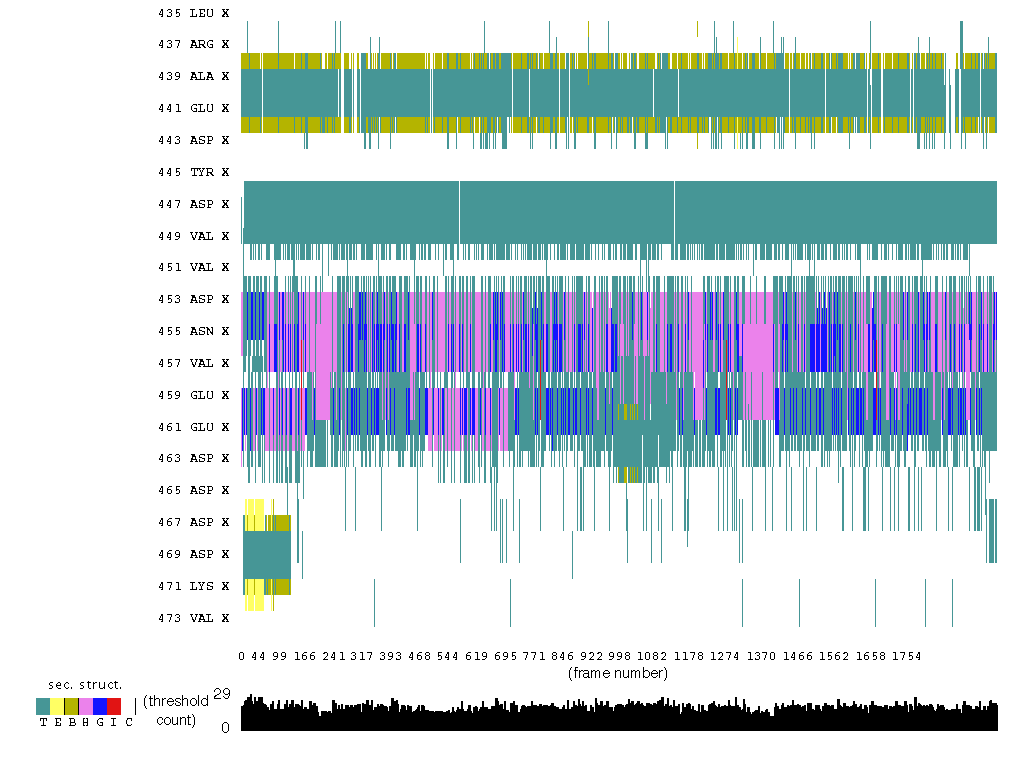
\includegraphics[width=0.49\textwidth]{wt_ss}}
	\subfigure[YD]{\label{fig:ss_b}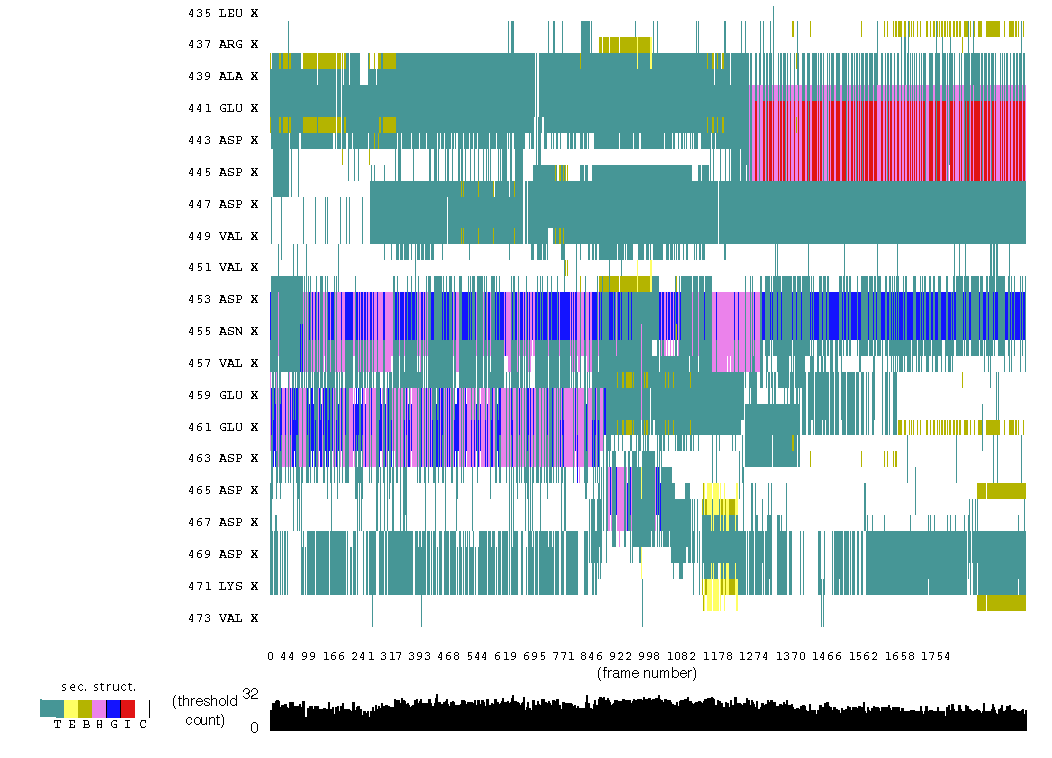
\includegraphics[width=0.49\textwidth]{yd_ss}}
	\FigureCaption{\gct Secondary Structure Assignments}{Per-residue secondary structure assignments based on 3D coordinates are computed for every frame of the simulation. WT and YD trajectories lack global and persistent secondary structure motifs throughout the duration of the simulation. Apart from turn motifs and small local $\alpha$-helices, the \gct samples largely disordered conformations and does not undergo any disorder-order transitions. T: turn, E: extended, B: isolated bridge, H: $\alpha$-helix, G: 3/10 Helix, I: $\pi$-helix, C: coil.}
	\label{fig:ss}
\end{figure}	


Although we do not observe ordered secondary structure rearrangements by looking at \texttt{dssp}, we compute RMSD to ask whether the simulations produce any conformational changes in the disordered ensemble. RMSD quantifies the distance between superimposed structures and is therefore a useful tool for detecting the presence of conformational changes in a trajectory. We therefore computed backbone RMSD values for every frame in the simulation with respect to the starting structure. Since the starting conformation is not derived from experimental data and is not expected to correspond to a native state, we also compute RMSD with a 10ns sliding window where every frame is compared with the one 10ns before. In the middle portion of the YD simulation, both methods of computing RMSD contain sharp peaks which indicate the presence of large scale backbone rearrangements \figref{fig:rmsd}. In contrast, WT RMSD values remain stable throughout the simulation. This suggests that the YD mutation can modulate conformational exploration and the stability of the \gct. 


\todo{RMSD figs}
\begin{figure}
	\centering     %%% not \center
	\subfigure[RMSD to initial frame]{\label{fig:a}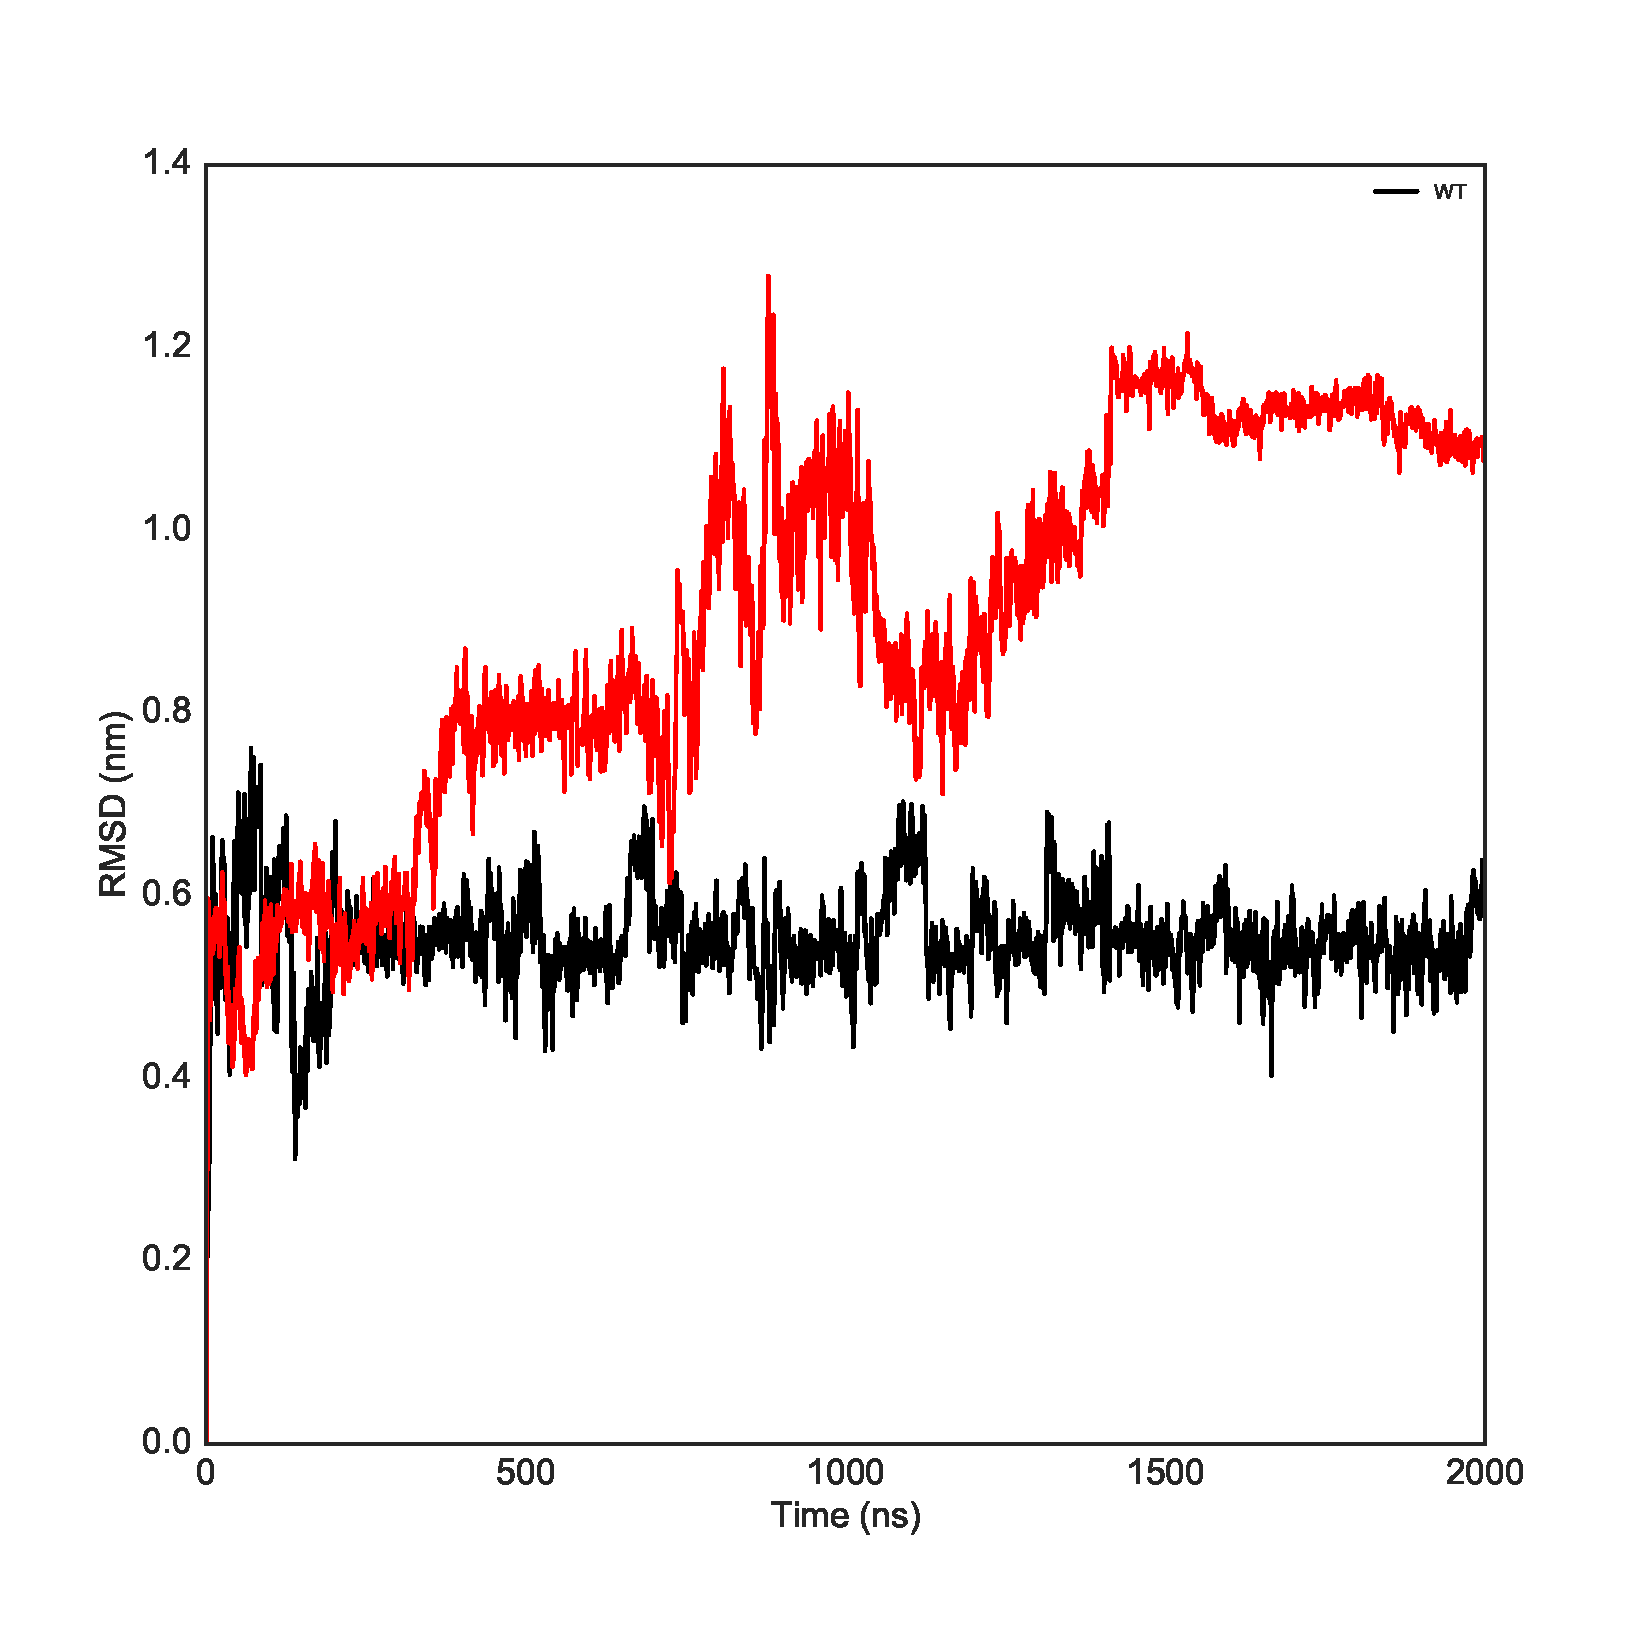
\includegraphics[width=0.49\textwidth]{rmsd}}
	\subfigure[RMSD 10ns window]{\label{fig:b}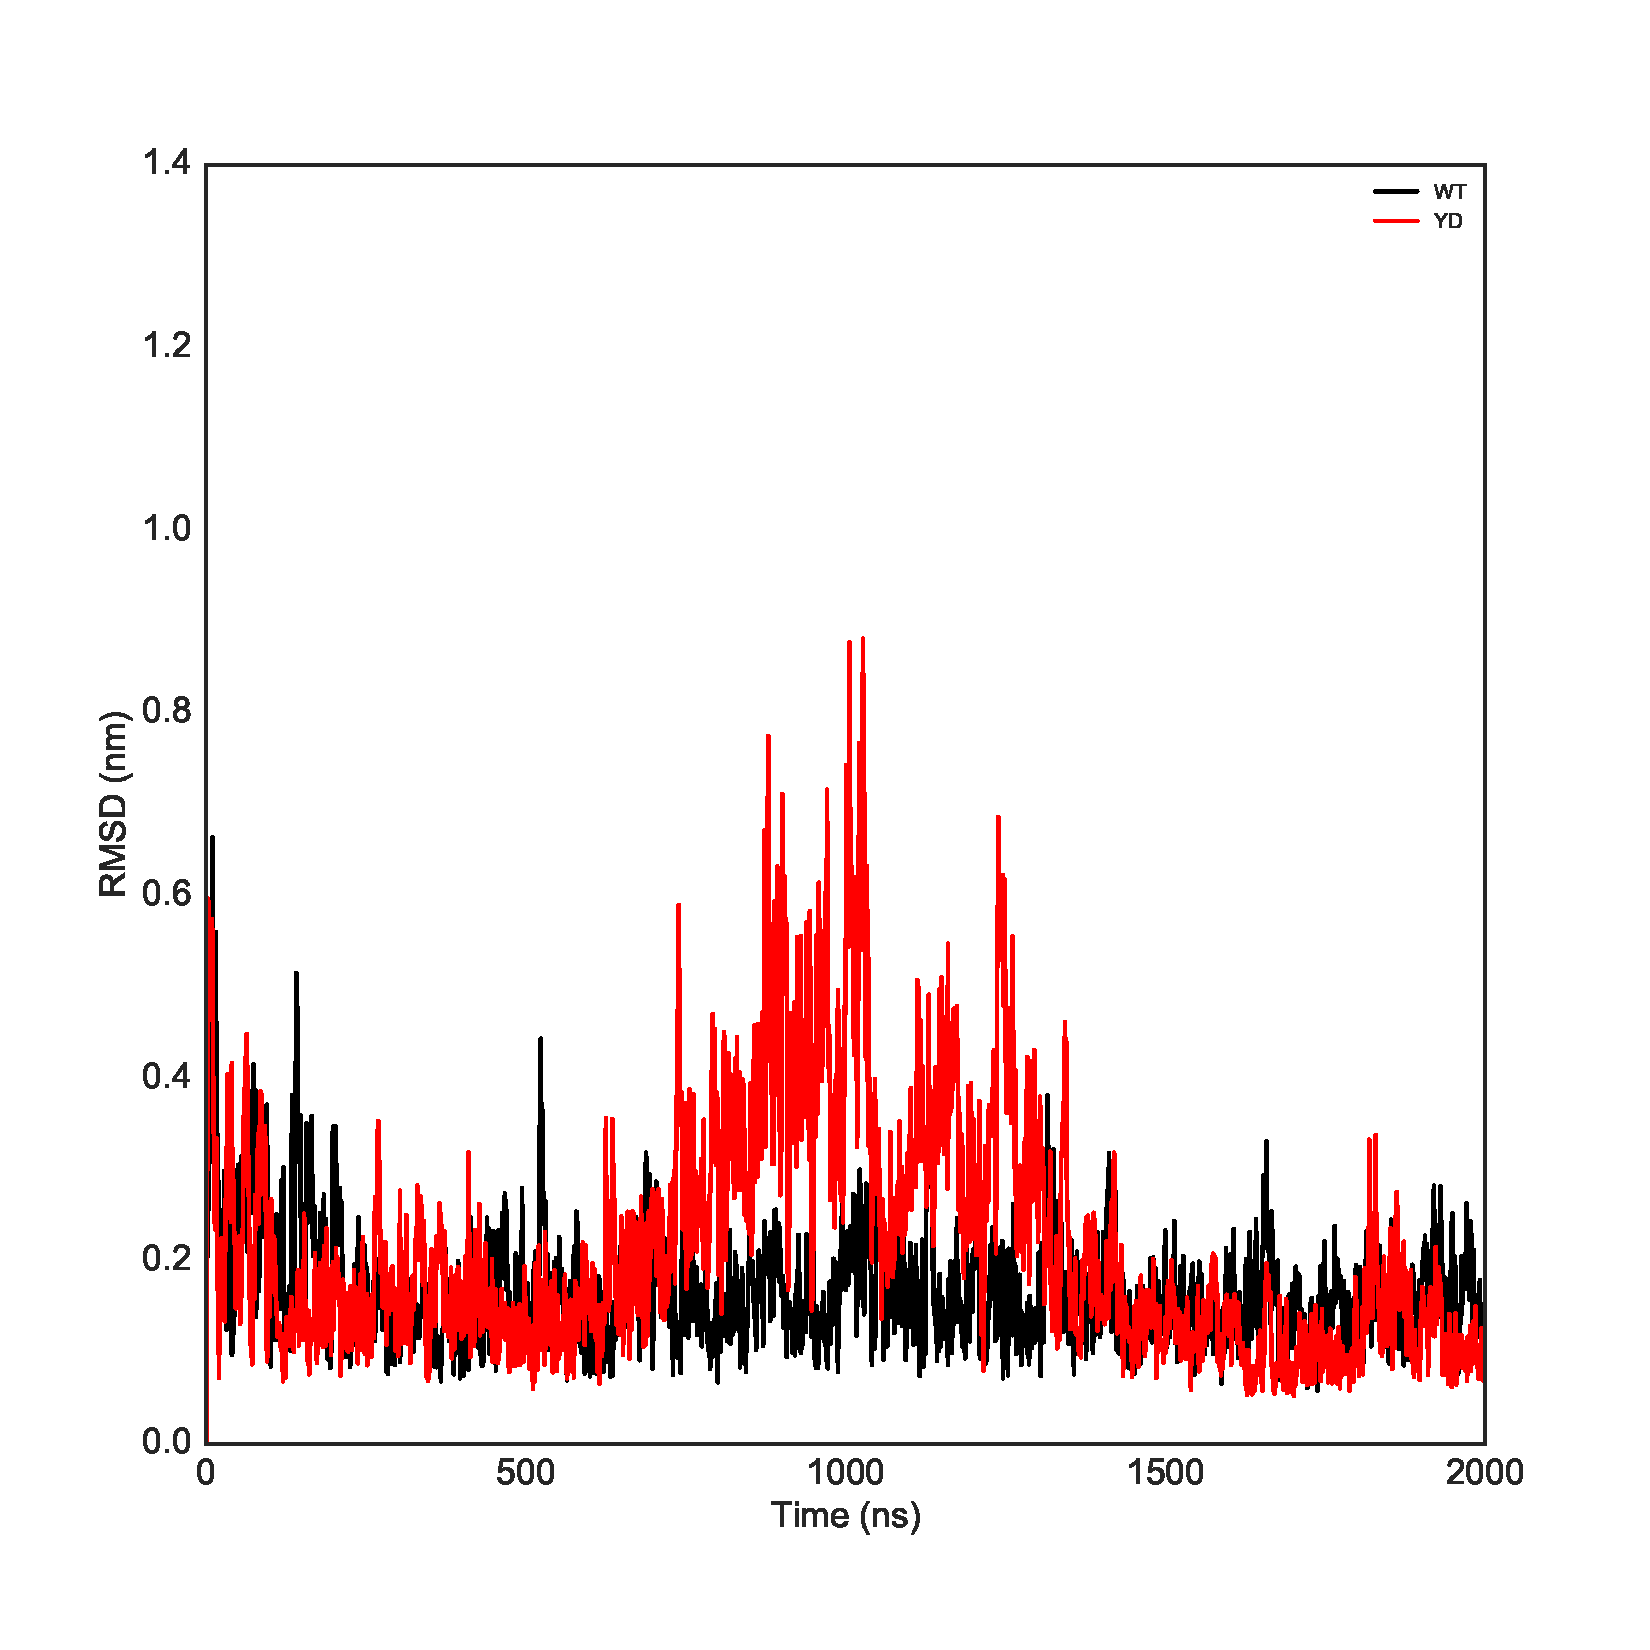
\includegraphics[width=0.49\textwidth]{rmsd_10}}
	\FigureCaption{RMSD}
	\label{fig:rmsd}
\end{figure}
	
{\it \gct is largely collapsed}

Given that NMR reports transitions between extended and collapsed conformations in the YD mutant, we hypothesize that a similar motion is driving the displacement observed in the RMSD computations. In order to obtain values of compactness that can be compared directly to NMR results, we compute the translational diffusion coefficient (\diffusion) of conformers in our simulations. As a reference point for interpreting the diffusion values of the trajectories, we use the software \texttt{flexiblemeccano} to compute an ensemble of disordered peptides of the YD polypeptide. \texttt{flexiblemeccano} takes a primary sequence as input and generates an ensemble of 3D conformations based on amino acid specific conformational potentials and volume exclusion. We then use \texttt{hydroNMR} to compute \diffusion values for each conformer and obtain a distribution for the \diffusion of the \gct. From this distribution \figref{fig:fm} we obtain a large range of conformations; from highly collapsed, to extended chains against which we can compare MD-derived values.

We computed global averages for the radius of gyration, and translational diffusion coefficient over the \SI{2}{\us} simulations. Both simulations appear to occupy largely collapsed conformations which agrees with experimental findings \figref{fig:dchist}. The WT polypeptide \diffusion mean is \diffusion = \num{1.237e-6} $\pm$ \SI{1.5816e-8}{\dcunits} while the value obtained through NMR is  \diffusion=\num{1.25e-6} $\pm$  \SI{1e-8}{\dcunits}. Similarly to what was seen by NMR, we find that the mean \diffusion of the Y445D \gct polypeptide is slightly lower than that of the WT \gct (\diffusion= \num{1.224e-6} $\pm$ \SI{3.503e-8}{\dcunits}). These results confirm that the \gct, while disordered, is more compact than a fully denatured polypeptide chain, and that the YD \gct is more extended on average.

\todo{chi square goodness of fit}

\todo{talk about benchmark for collapsed state}

\begin{figure}
	\centering     %%% not \center
	\subfigure[Distribution of \diffusion in conformer ensemble]{\label{fig:fmdist}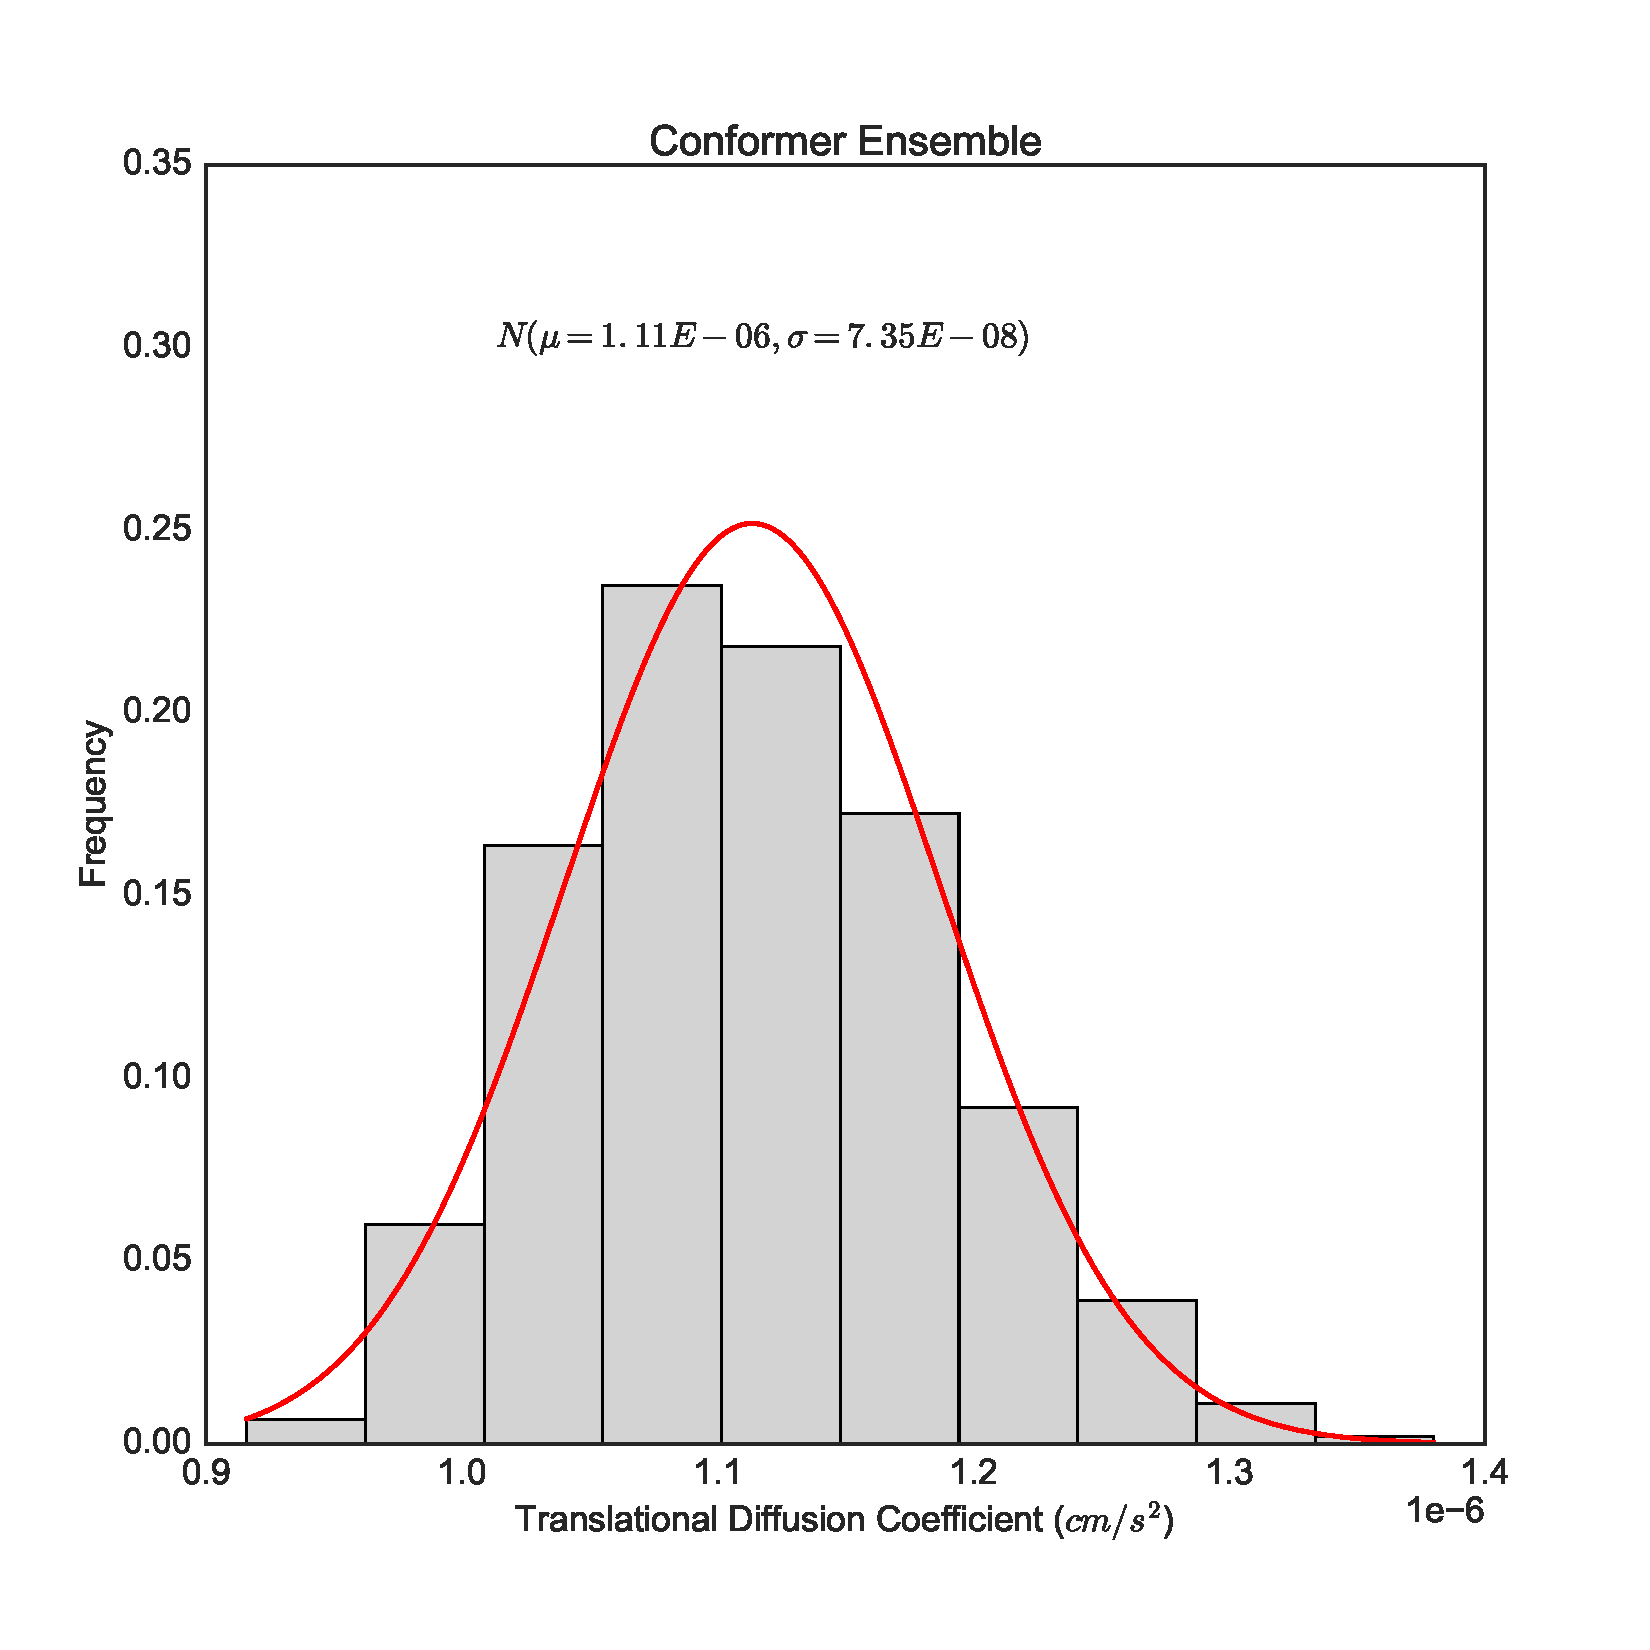
\includegraphics[width=0.49\textwidth]{FM_hist}}
	\subfigure[Representative structures]{\label{fig:rainbows}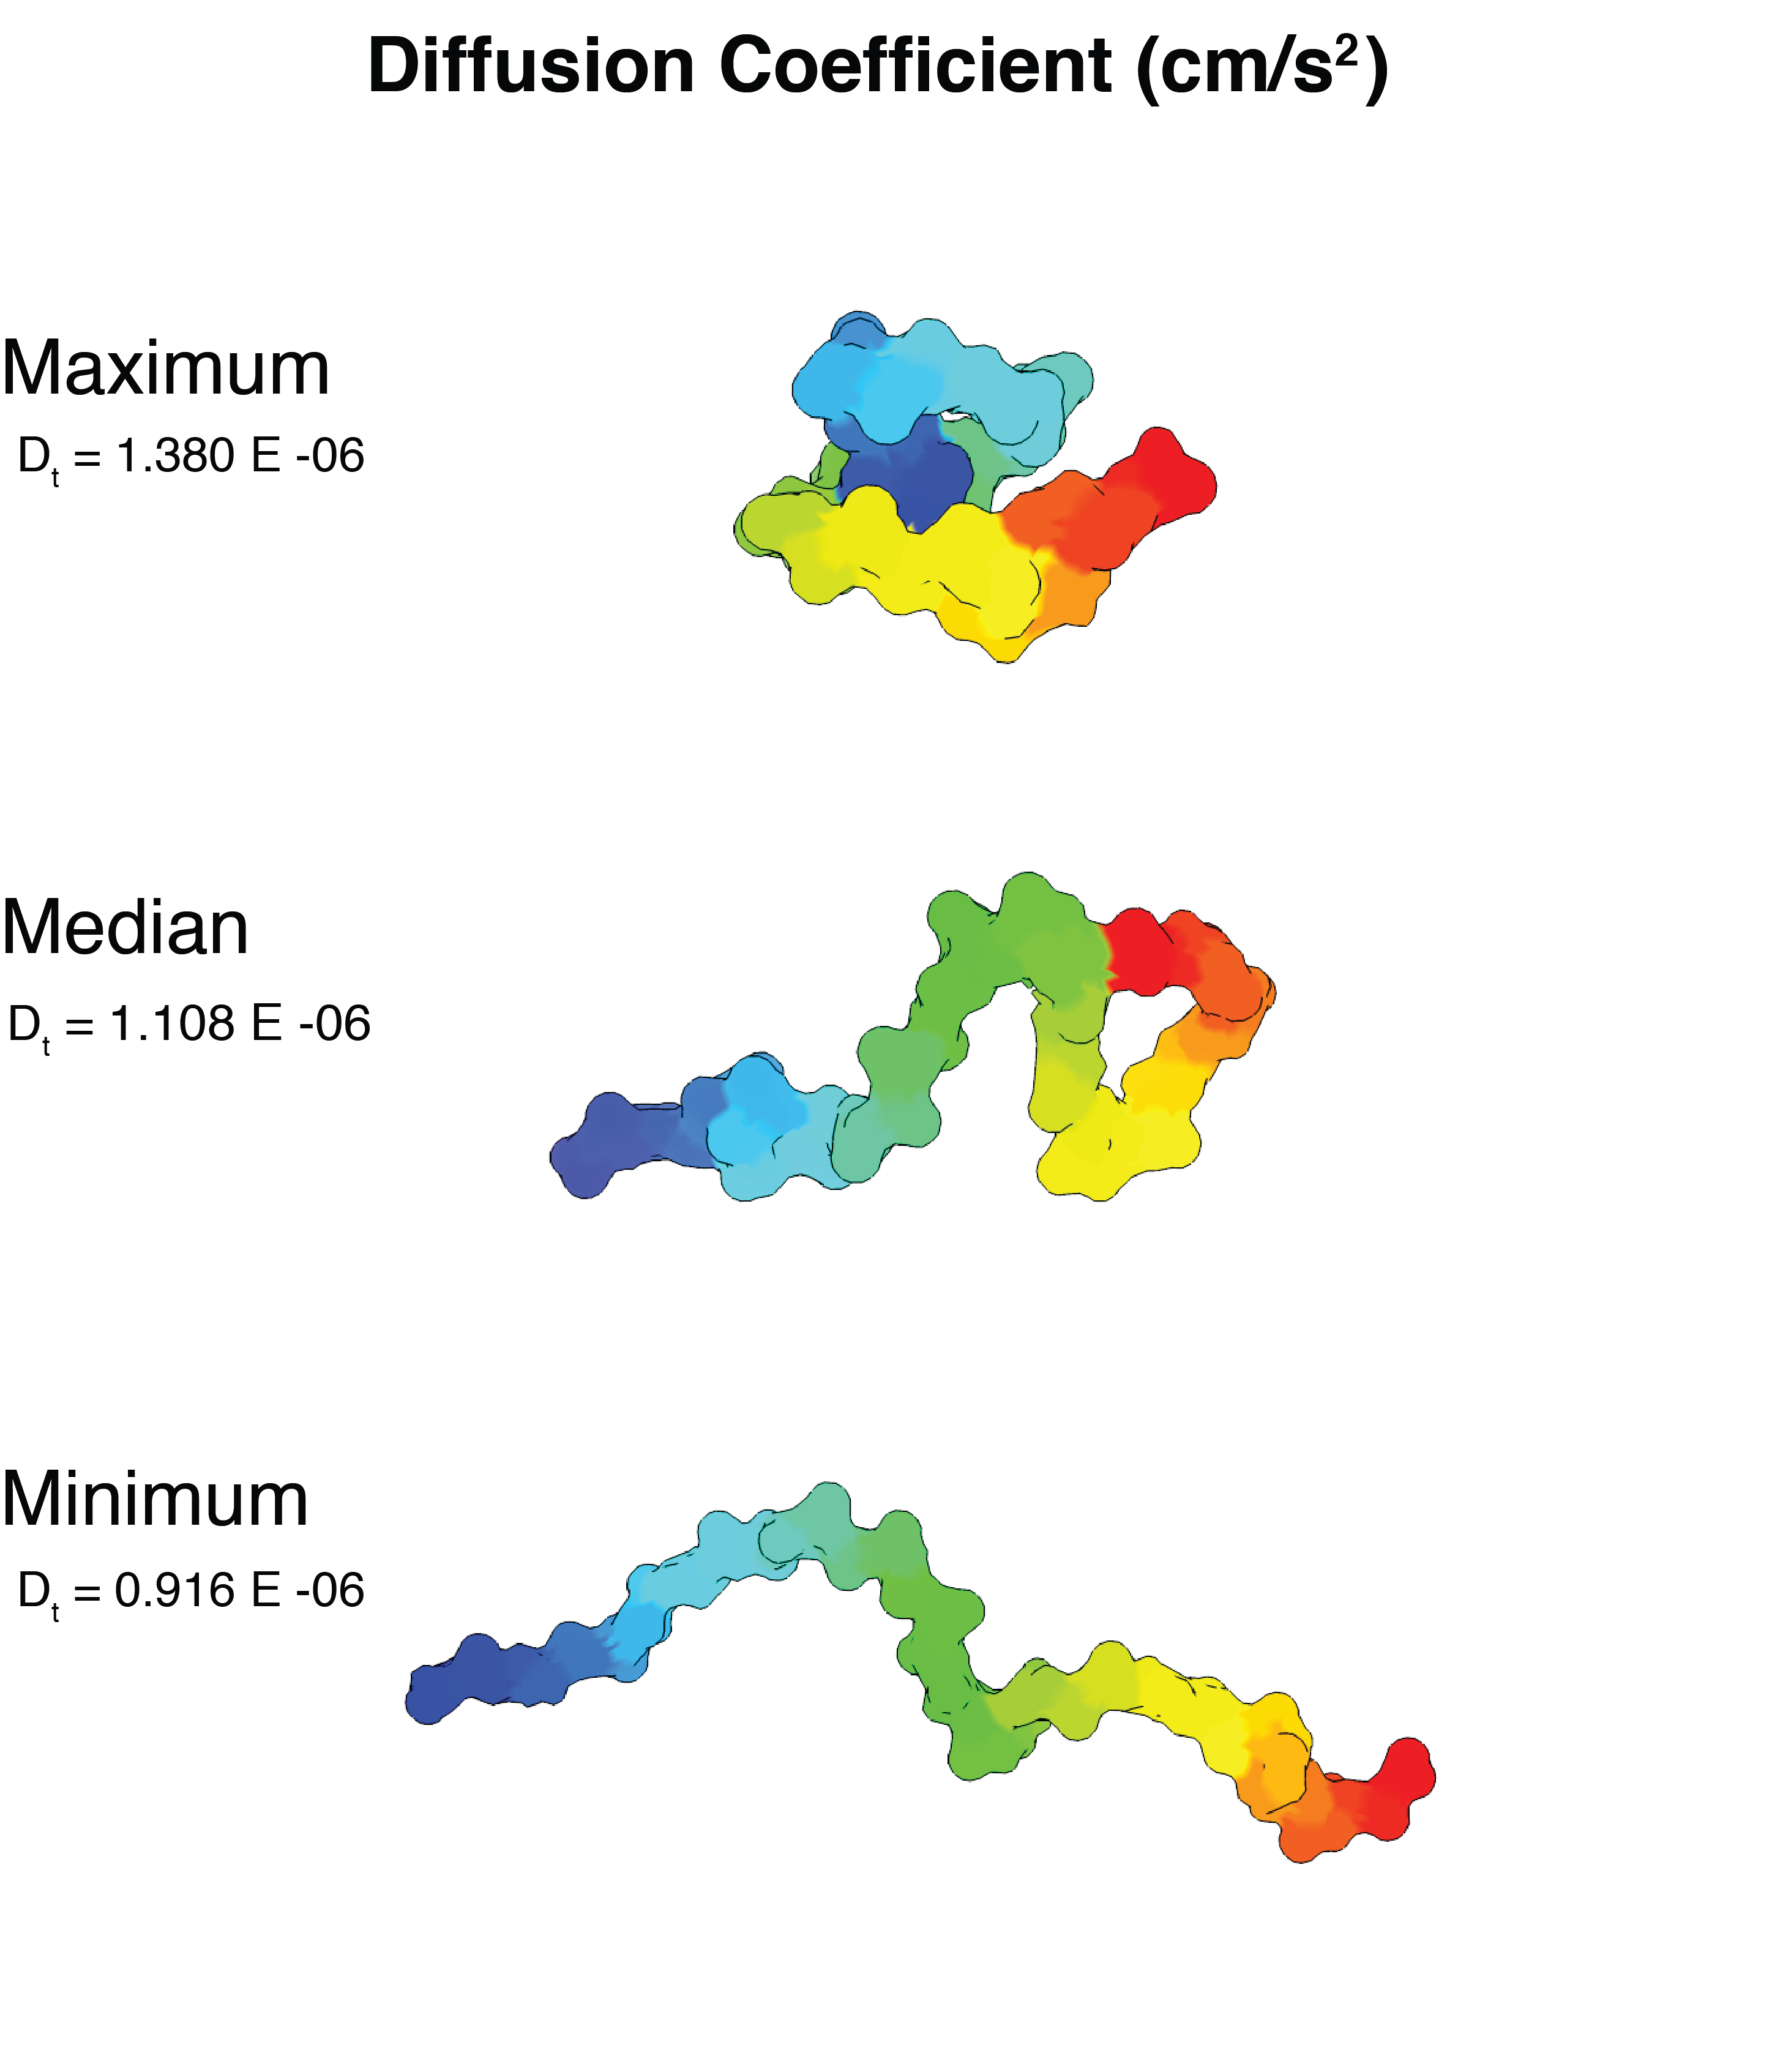
\includegraphics[height=0.35\textheight]{FM_rainbows}}
	\FigureCaption{\gct predicted conformational ensemble}{We use \texttt{flexiblemeccano} to obtain a conformer ensemble based on the primary sequence of the \gct and plot \diffusion for every conformer in the set of 10,000 sampled structures \figref{fig:fmdist}. We visualize the structures corresponding to the maximum, minimum, and median \diffusion. \figref{fig:rainbows}}
	\label{fig:fm}
\end{figure}

Translational diffusion coefficient measurements in NMR report that both \gct forms primarily occupy collapsed conformations. The global experimental average for the WT polypeptide obtained through NMR is \diffusion=\num{1.25e-6} $\pm$  \SI{1e-8}{\dcunits} which agrees well with the NMR-derived value (\diffusion=\num{1.25e-6} $\pm$  \SI{1e-8}{\dcunits}. Similarly to what was seen by NMR, we find that the mean \diffusion of the Y445D \gct polypeptide is slightly lower than that of the WT \gct (\diffusion= \num{1.224e-6} $\pm$ \SI{3.503e-8}{\dcunits}). These results confirm that the \gct, while disordered, is more compact than a fully denatured polypeptide chain \figref{fig:dclines}. 

Although both forms of the \gct primarily occupy collapsed and disordered conformations, we do observe that, as in NMR, the YD \gct has a slightly lower mean \diffusion than WT. From NMR we hypothesize that this is caused by transitions between compacted and extended driven by enhanced dynamics in the YD mutant. Lending support to this hypothesis, we show that we are able to explain the distribution of diffusion coefficients in the YD mutant as the sum of two gaussian distributions with parameters $\mu_1 =\SI{1.24e-6}{\dcunits}, \sigma_2= \num{2.34e-8}, \mu_2 =\SI{1.18e-6}{\dcunits}, \sigma_2= \num{2.21e-8}$ \figref{fig:dchistyd}. This suggests that the YD dynamics likely give rise to a two-state system where a minor state occupies extended conformations \figref{fig:dclines}. Meanwhile, the WT \diffusion distribution is best explained by a single normal distribution which suggests that the peptide occupies a single stable state which corresponds to the compacted portion of conformation space \figref{fig:dchistwt}.

\begin{figure}
\centering     %%% not \center
\subfigure[Figure A]{\label{fig:dchistwt}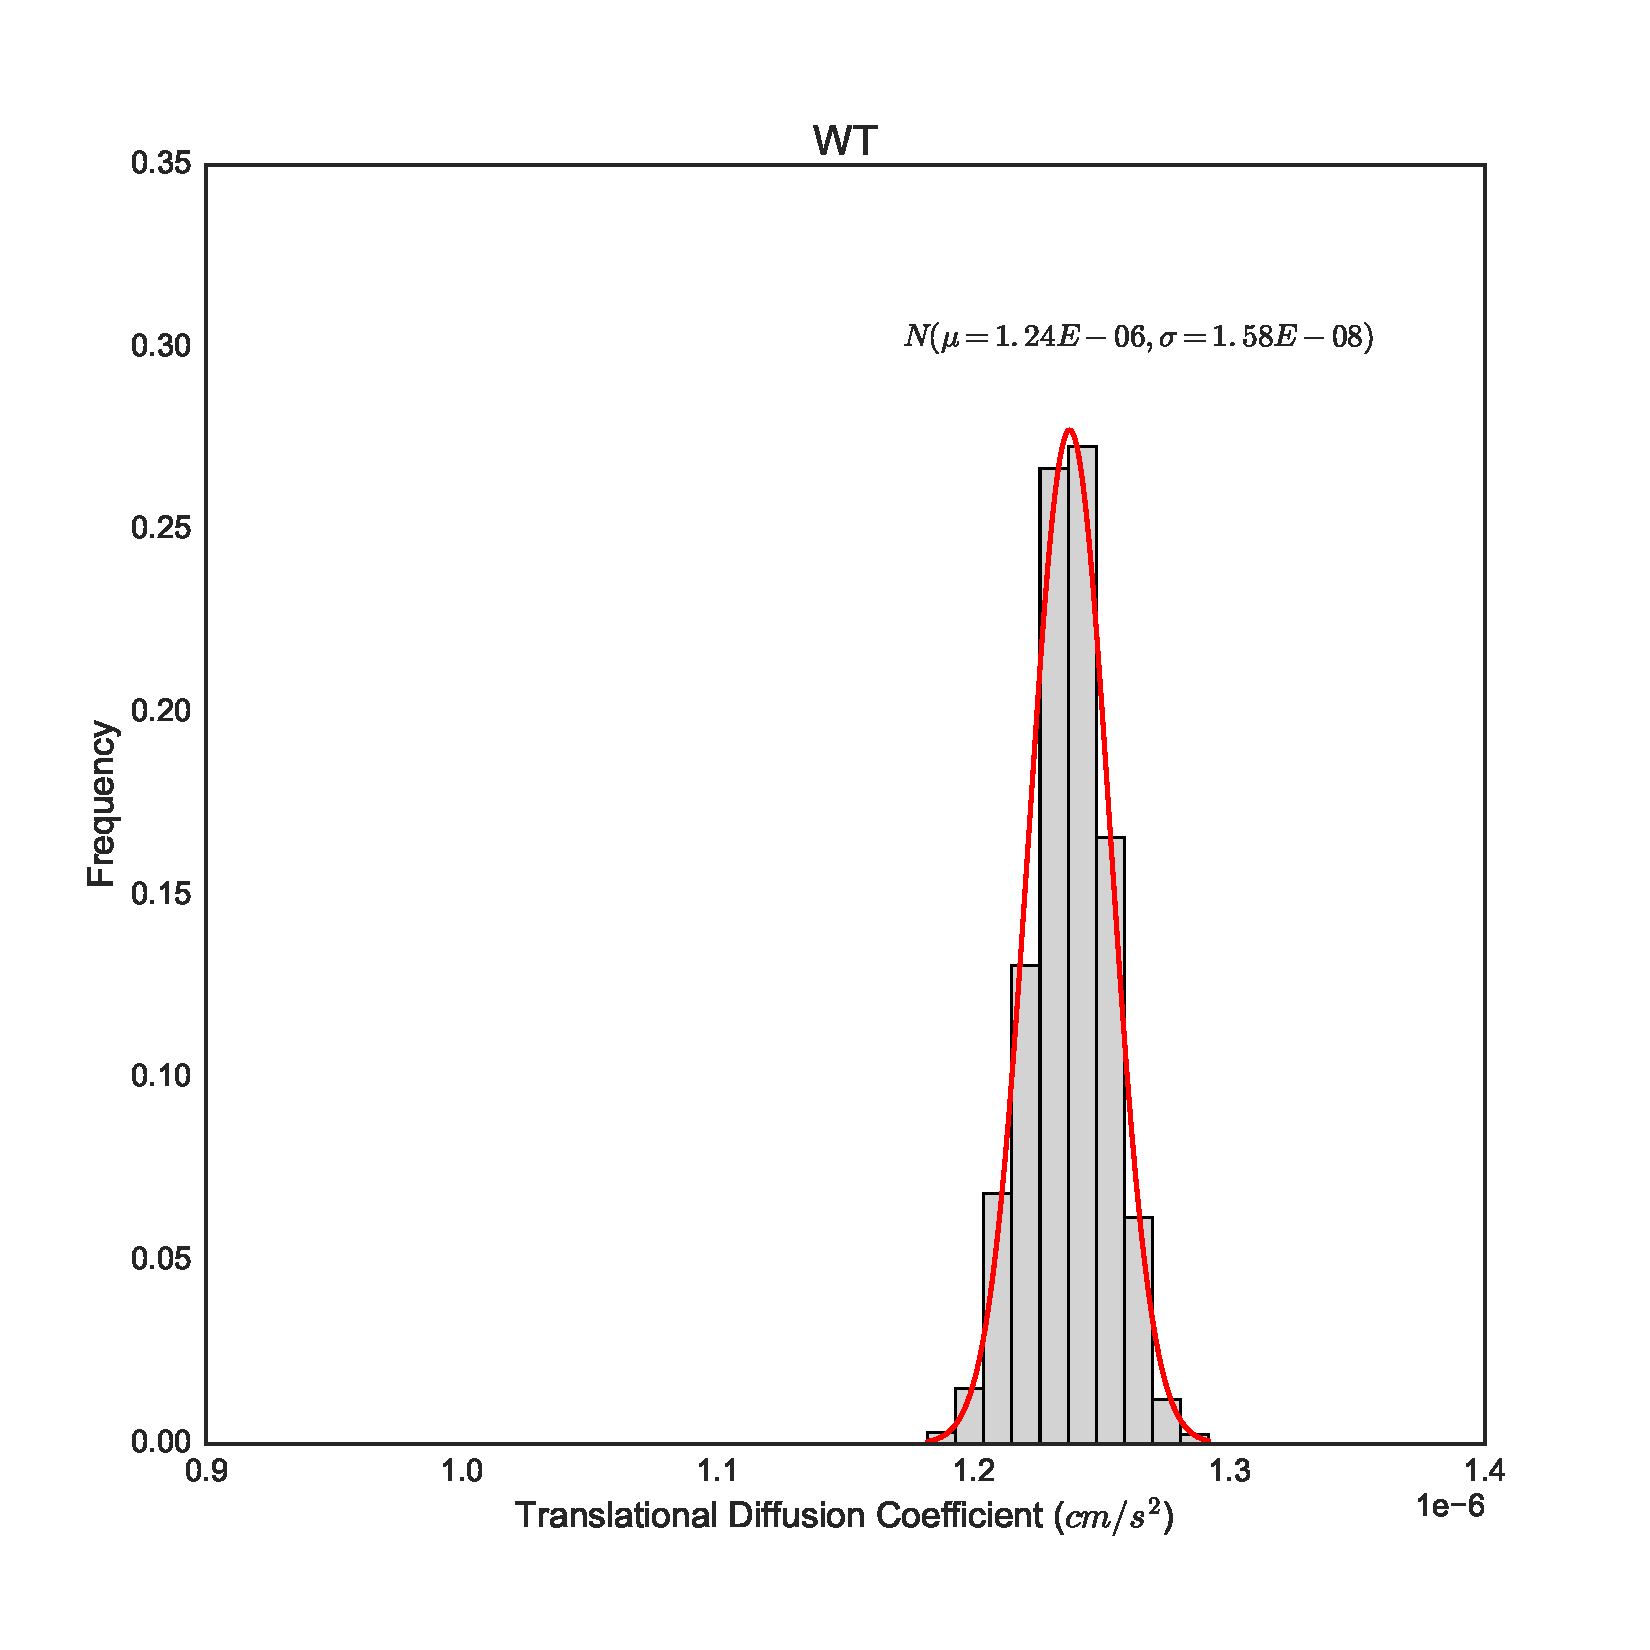
\includegraphics[width=0.49\textwidth]{wt_hist}}
\subfigure[Figure B]{\label{fig:dchistyd}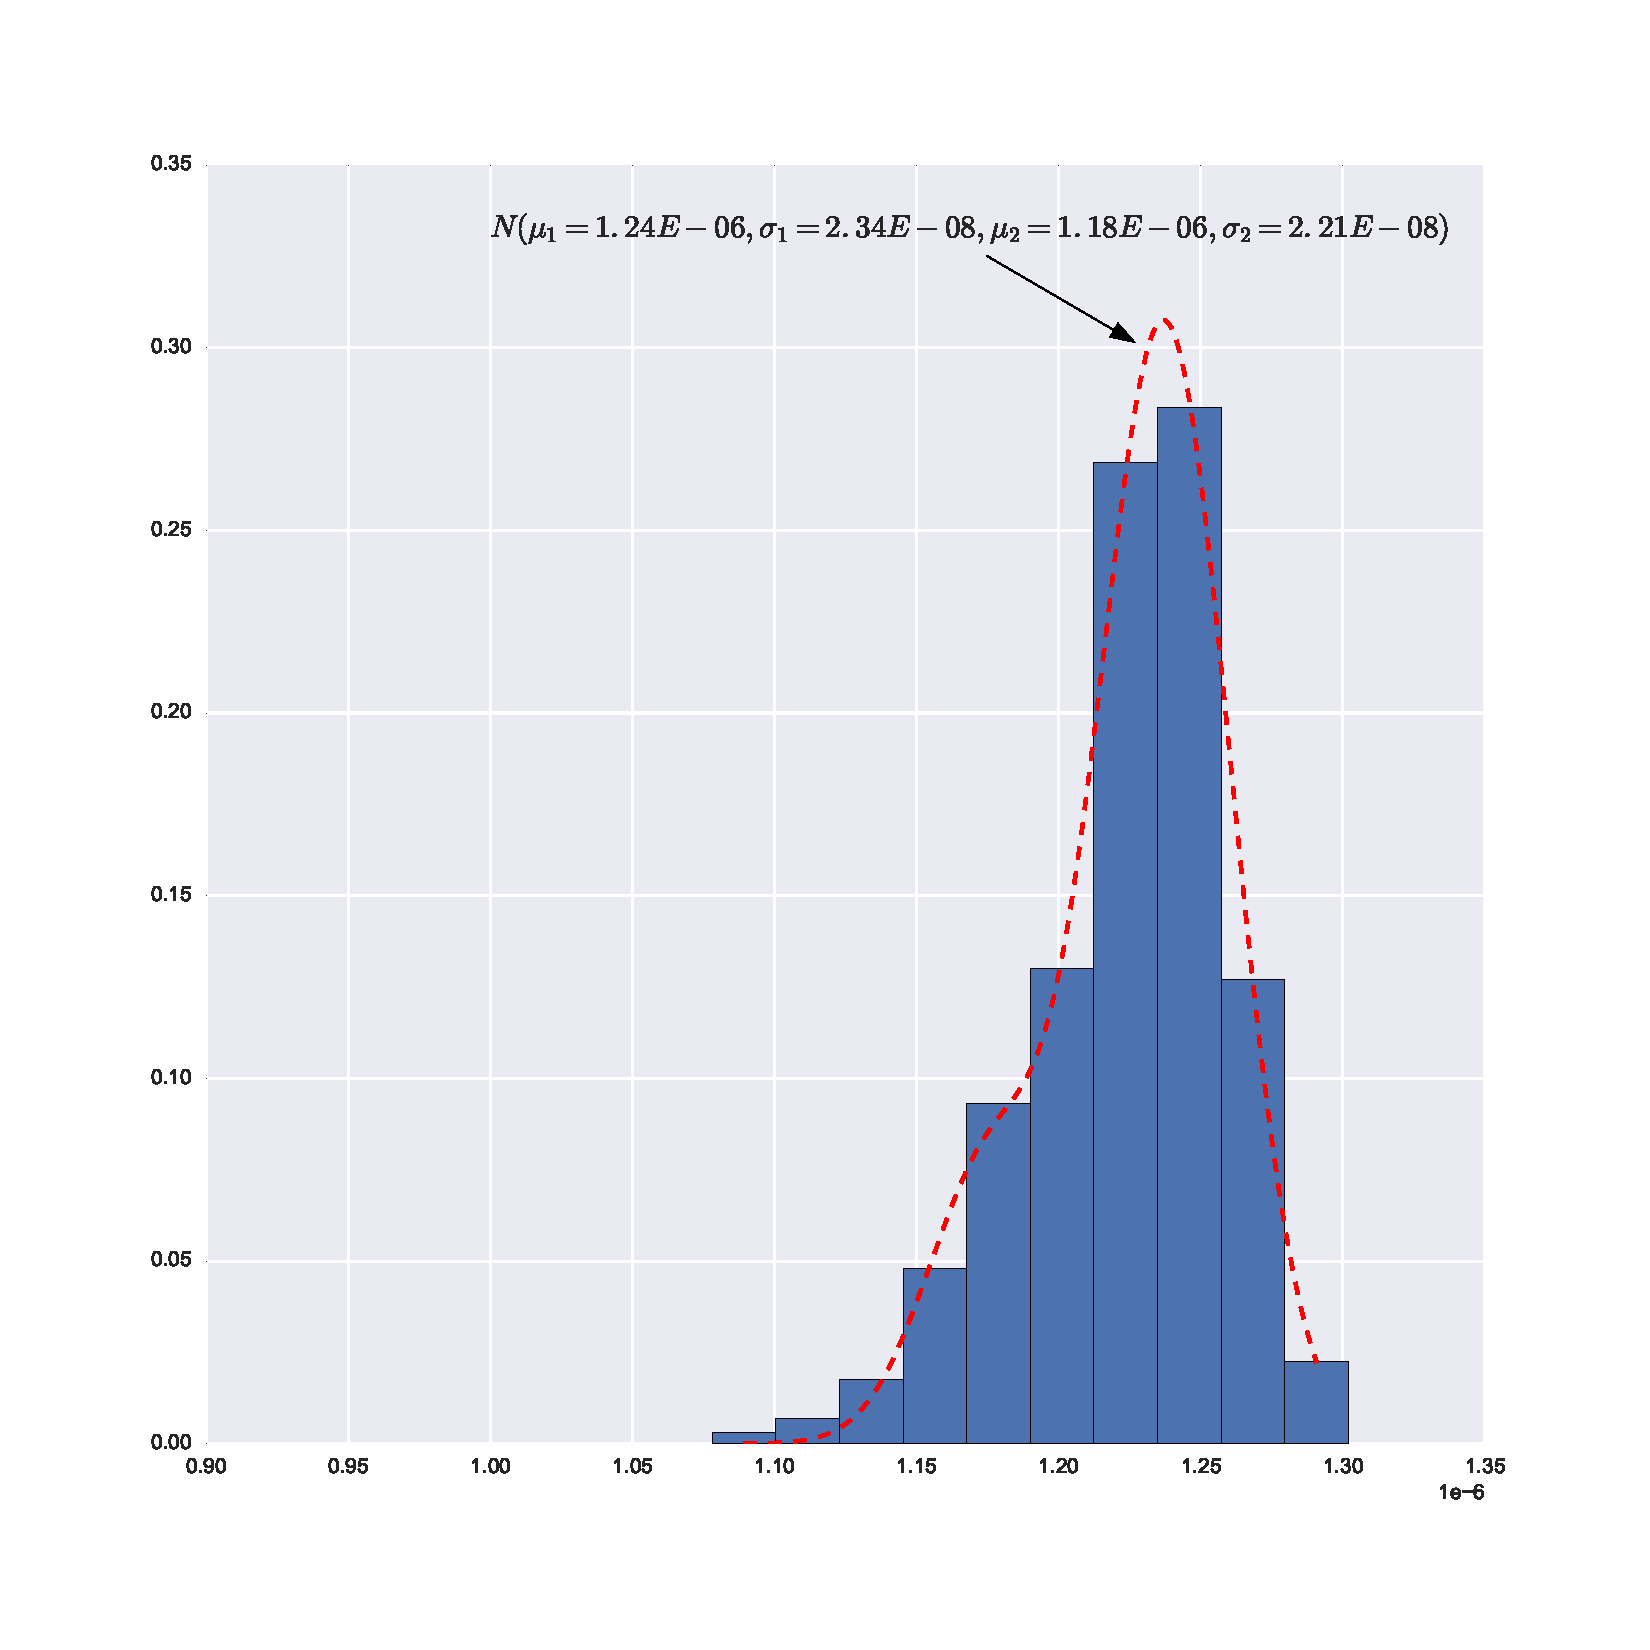
\includegraphics[width=0.49\textwidth]{yd_2gauss}}
\subfigure[Figure C]{\label{fig:dclines}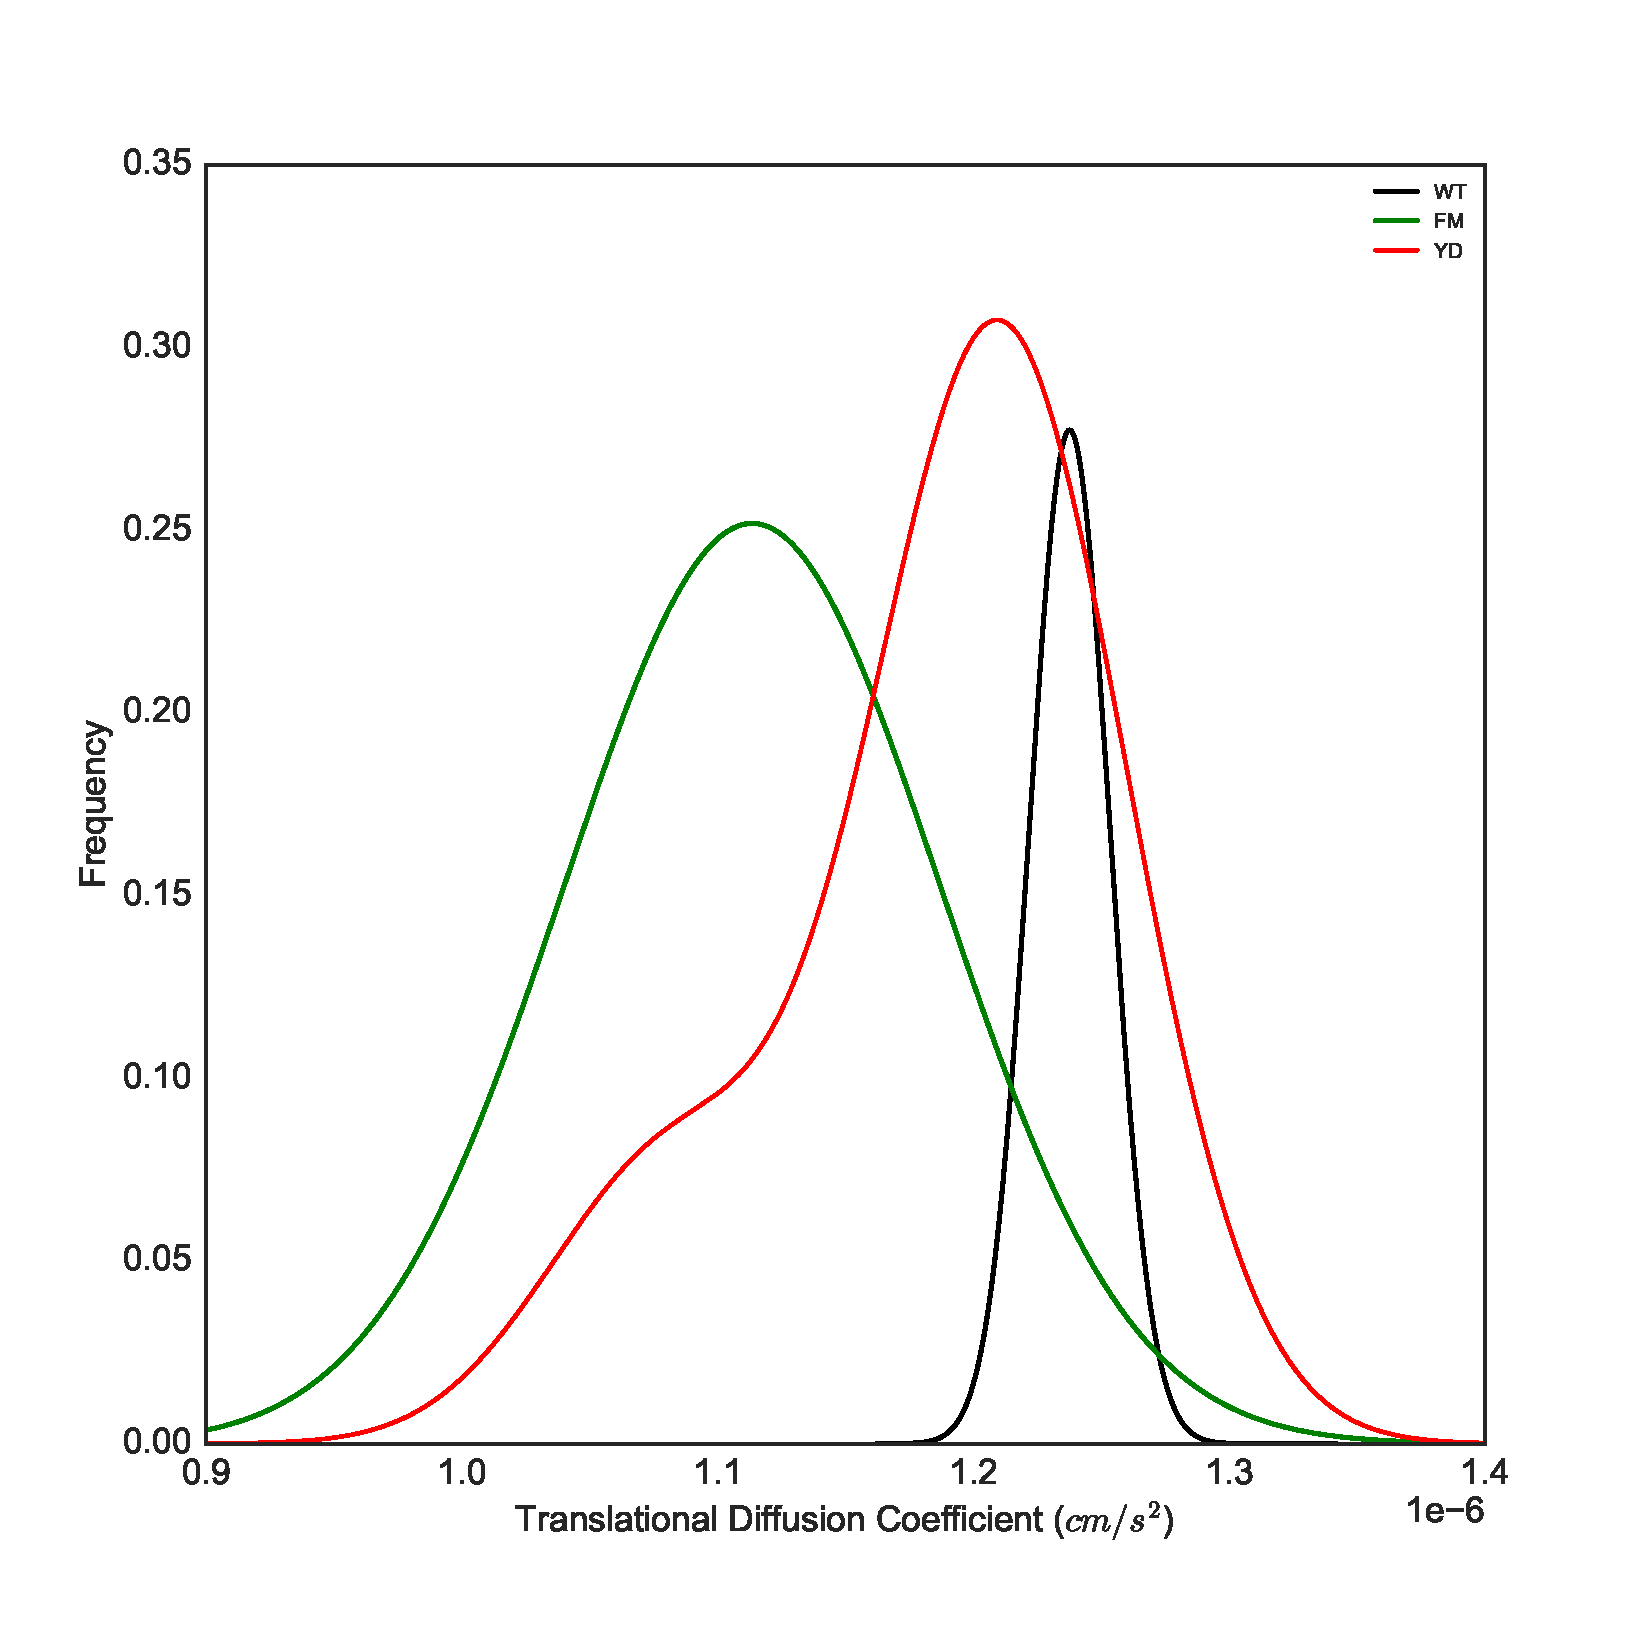
\includegraphics[width=0.49\textwidth]{lines_dc}}
\FigureCaption{Distribution of diffusion coefficients}
\label{fig:dchist}
\end{figure}



\begin{figure}
	\centering     %%% not \center
	\subfigure[\diffusion over simulation time]{\label{fig:a}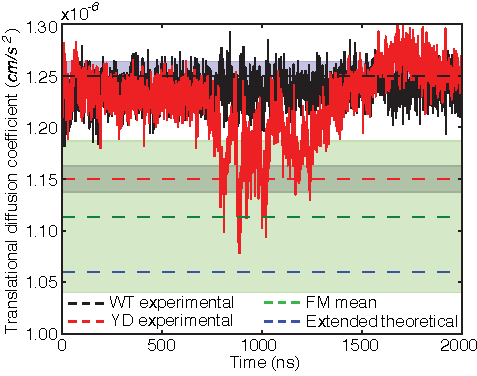
\includegraphics[height=0.35\textheight]{dc_ts}}
	\subfigure[Representative structures]{\label{fig:b}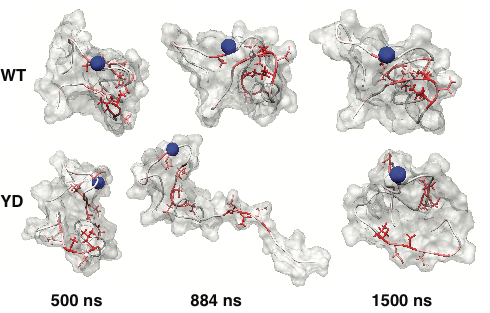
\includegraphics[height=0.3\textheight]{dc_strucs}}
	\FigureCaption{Secondary structure assignments}
	\label{fig:dctime}
\end{figure}

Looking at \diffusion as a function of simulation time, we found that the diffusion coefficient (\diffusion) of the WT \gct remains relatively constant throughout the simulation, (\diffusion = \num{1.237e-6} $\pm$ \SI{1.5816e-8}{\dcunits} and agrees well with the NMR-derived value (\diffusion=\num{1.25e-6} $\pm$  \SI{1e-8}{\dcunits}.  Similarly to what was seen by NMR, we find that the mean \diffusion of the Y445D \gct polypeptide is slightly lower than that of the WT \gct (\diffusion= \num{1.224e-6} $\pm$ \SI{3.503e-8}{\dcunits}). These results confirm that the \gct, while disordered, is more compact than a fully denatured polypeptide chain. Interestingly, between \num{762} to \SI{1255}{\ns} in the MDS, the Y445D \gct underwent transient excursions to less compact con-formations with significantly lower diffusion coefficients (mean \diffusion= \num{1.152e-6} $\pm$ \SI{2.0325e-8}{\dcunits}). This sub-population is more extended (i.e. diffuses more slowly) than any conformation sampled by the WT \gct throughout the entire MDS. While the Y445D \gct extended states do not overlap with the conformational ensemble of the WT \gct polypeptides, they do, however, lie close to the extended conformational space for a typical random-coil poly-peptide, as modeled by \texttt{flexiblemeccano} \figref{fig:dctime}.

In order to visualize a non-overlapping subset of conformations to represent extended and collapsed states, we use the \diffusion distributions in \figref{fig:dchist} to select the conformations within the top and bottom 1\% (20 structures each) of the WT \gct and Y445D \gct. In the case of the WT, we do not expect the upper and lower \diffusion subsets to substantially differ, as the WT \gct conformations exhibit fairly homogeneous compactness overall. For Y445D \gct, we expect the upper \diffusion subset to resemble that of the WT \gct, while the lower \diffusion subset is expected to reflect the transient opening process. We plotted the mean distance between alpha carbons of all pairs of residues as contact maps for the set of collapsed (upper) and extended (lower) conformations of the WT \gct polypeptide \figref{fig:wt_contacts} and the Y445D \gct polypeptide \figref{fig:yd_contacts}.   As expected, the upper and lower \diffusion subsets of the WT \gct and the upper Ds subset of the YD \gct polypeptides show similar patterns of pair-wise contacts.  In contrast, the C-terminal residues in the lower \diffusion subset of the Y445D \gct lose the majority of contacts with N terminal residues, as a consequence of the conformational expansion. Next, we isolated the three conformations from the upper and lower \diffusion subsets of  Y445D \gct poly-peptides with the lowest all-to-all RMS, also known as centroid structures, shown in \figref{fig:representatives} with large relaxation dispersion magnitudes indicated in red. This analysis shows that the extended conformations consist of a compact N-terminus with residues located in the C-terminal region of the \gct, (including dynamically-broadened residues L30, A32 and G34) isolated from the N-terminus and solvent-accessible. Through MD we are able to re-produce the anomalously rapid diffusion (i.e. high compactness) of the WT and Y445D ground-state \gct polypeptides. Moreover, we saw that the YD substitution caused relatively slow collective motions of the entire polypeptide chain, as observed by NMR. This provides a possible explanation for how residues throughout a disordered polypeptide can experience a concerted, two-state, dynamical process presence of the Y445D mutation, and suggests that it is the separation of a cluster of residues located in N and C termini of the \gct polypeptide that drives a transition to extended conformations with a concomitant  reduction of the translational diffusion coefficient.


\begin{figure}
\centering     %%% not \center
\subfigure[Figure A]{\label{fig:wt_contacts}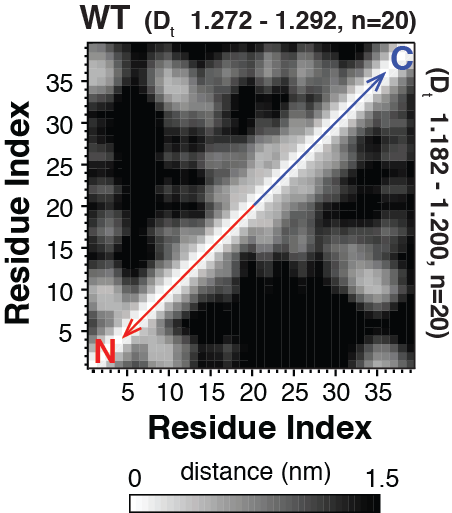
\includegraphics[width=0.49\textwidth]{wt_contacts}}
\subfigure[Figure B]{\label{fig:yd_contacts}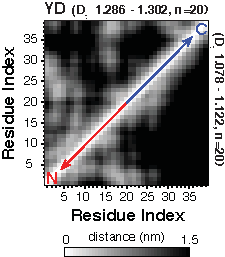
\includegraphics[width=0.49\textwidth]{yd_contacts}}
\subfigure[Figure C]{\label{fig:representatives}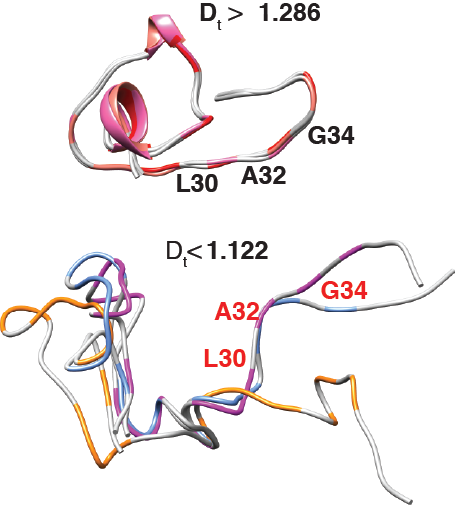
\includegraphics[width=0.49\textwidth]{representatives}}
\FigureCaption{Distribution of diffusion coefficients}
\label{fig:contacts}
\end{figure}




\begin{figure}
\centering     %%% not \center
\subfigure[Figure A]{\label{fig:a}\includegraphics[width=0.7\textwidth]{glob_overlay}}
\subfigure[Figure B]{\label{fig:b}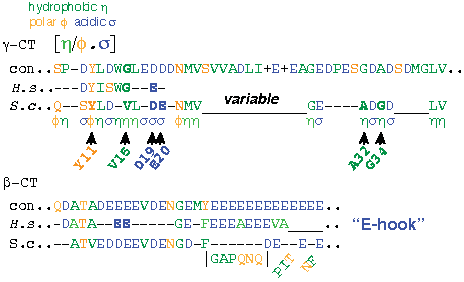
\includegraphics[width=0.7\textwidth]{consensus}}
\end{figure}

\subsection{Collective motions correspond to transitions between extended and collapsed conformations}

Until this point, we have identified the presence of an extended sub-population of the YD \gct that is absent in the WT. This lends support to the hypothesis that the shift in \diffusion measured by NMR is due to transient expansions of the YD backbone into an extended state. Complementary to this finding, is the fact that residues in the YD polypeptide show evidence of collective motions detected as shifts in chemical environment through NMR \todo{r2 figure appendix} which suggest that the transition between states occurs in a coordinated manner. We therefore seek to test whether correlated motions are also present in the simulation, and if they are, whether they can explain the transitions between collapsed and extended states.

We performed covariance analysis, also known as Principal Component Analysis on \gct trajectories to identify major axes of correlated motion. We use \texttt{covar} and \texttt{anaeig} from the \texttt{GROMACS} package to build a covariance matrix for backbone atoms to extract principal modes and perform eigenvector projections. In order to eliminate rotational and diffusive \todo{look this up} translations we align all frames in the trajectory to the average structure as computed by \texttt{covar} using RMSD based clustering. As is typical with molecular simulations which operate on a limited number of degrees of freedom, the first few eigenvectors in both trajectories account for nearly all of the variation in the trajectories \figref{fig:eigenvalues}. We therefore focus our attention on the two first major modes of motion. \todo{time plot of projections in major components}. \figref{fig:pca} shows a 2 dimensional projection onto the first two eigenvalues of WT and YD trajectories. Each point represents a 3D conformation in the \SI{2}{\us} simulation projected along the first two eigenvectors. The WT projection shows a conformational space that is closely clustered, indicative of constrained motions which is consistent with the low dispersions found in NMR and the single state behaviour suggested by RMSD and \diffusion analysis. However, the YD appears to be exploring  multiple conformation clusters which is in agreement with the presence of high dispersion groups found in NMR. Furthermore, by coloring each conformation with a normalized \diffusion value we are able to show that correlated motions along the major modes correspond with transitions between collapsed and extended states. In order to visualize the transitions, we generate a porcupine plot depicting the direction of motion between conformations on two extremes of the second principal component projections \figref{fig:porcupine}.  We show that the transition between collapsed and extended is indeed driven by a separation of the N and C terminus in a correlated fashion. \todo{cosine content} With this analysis we are able to propose a physical mechanism to explain the concerted global dynamics and diffusion coefficient shift observed in NMR as the action of correlated motions brought about by a local change in electrostatic environment. This physical mechanism would be the first example of an organized regulatory switch that does not count on disorder-order transitions but rather remains in the disordered ensemble. 

%When choosing which component to use for the visualization we computed cosine content values of each projection. This has been shown to be an effective method for detecting the presence of diffusion in signals from trajectories which often dominate the first few eigenvectors. The only component with significantly high cosine content was the first principal component of the YD simulation and so we focus our attention on projections along the second component.




\begin{figure}
\centering
	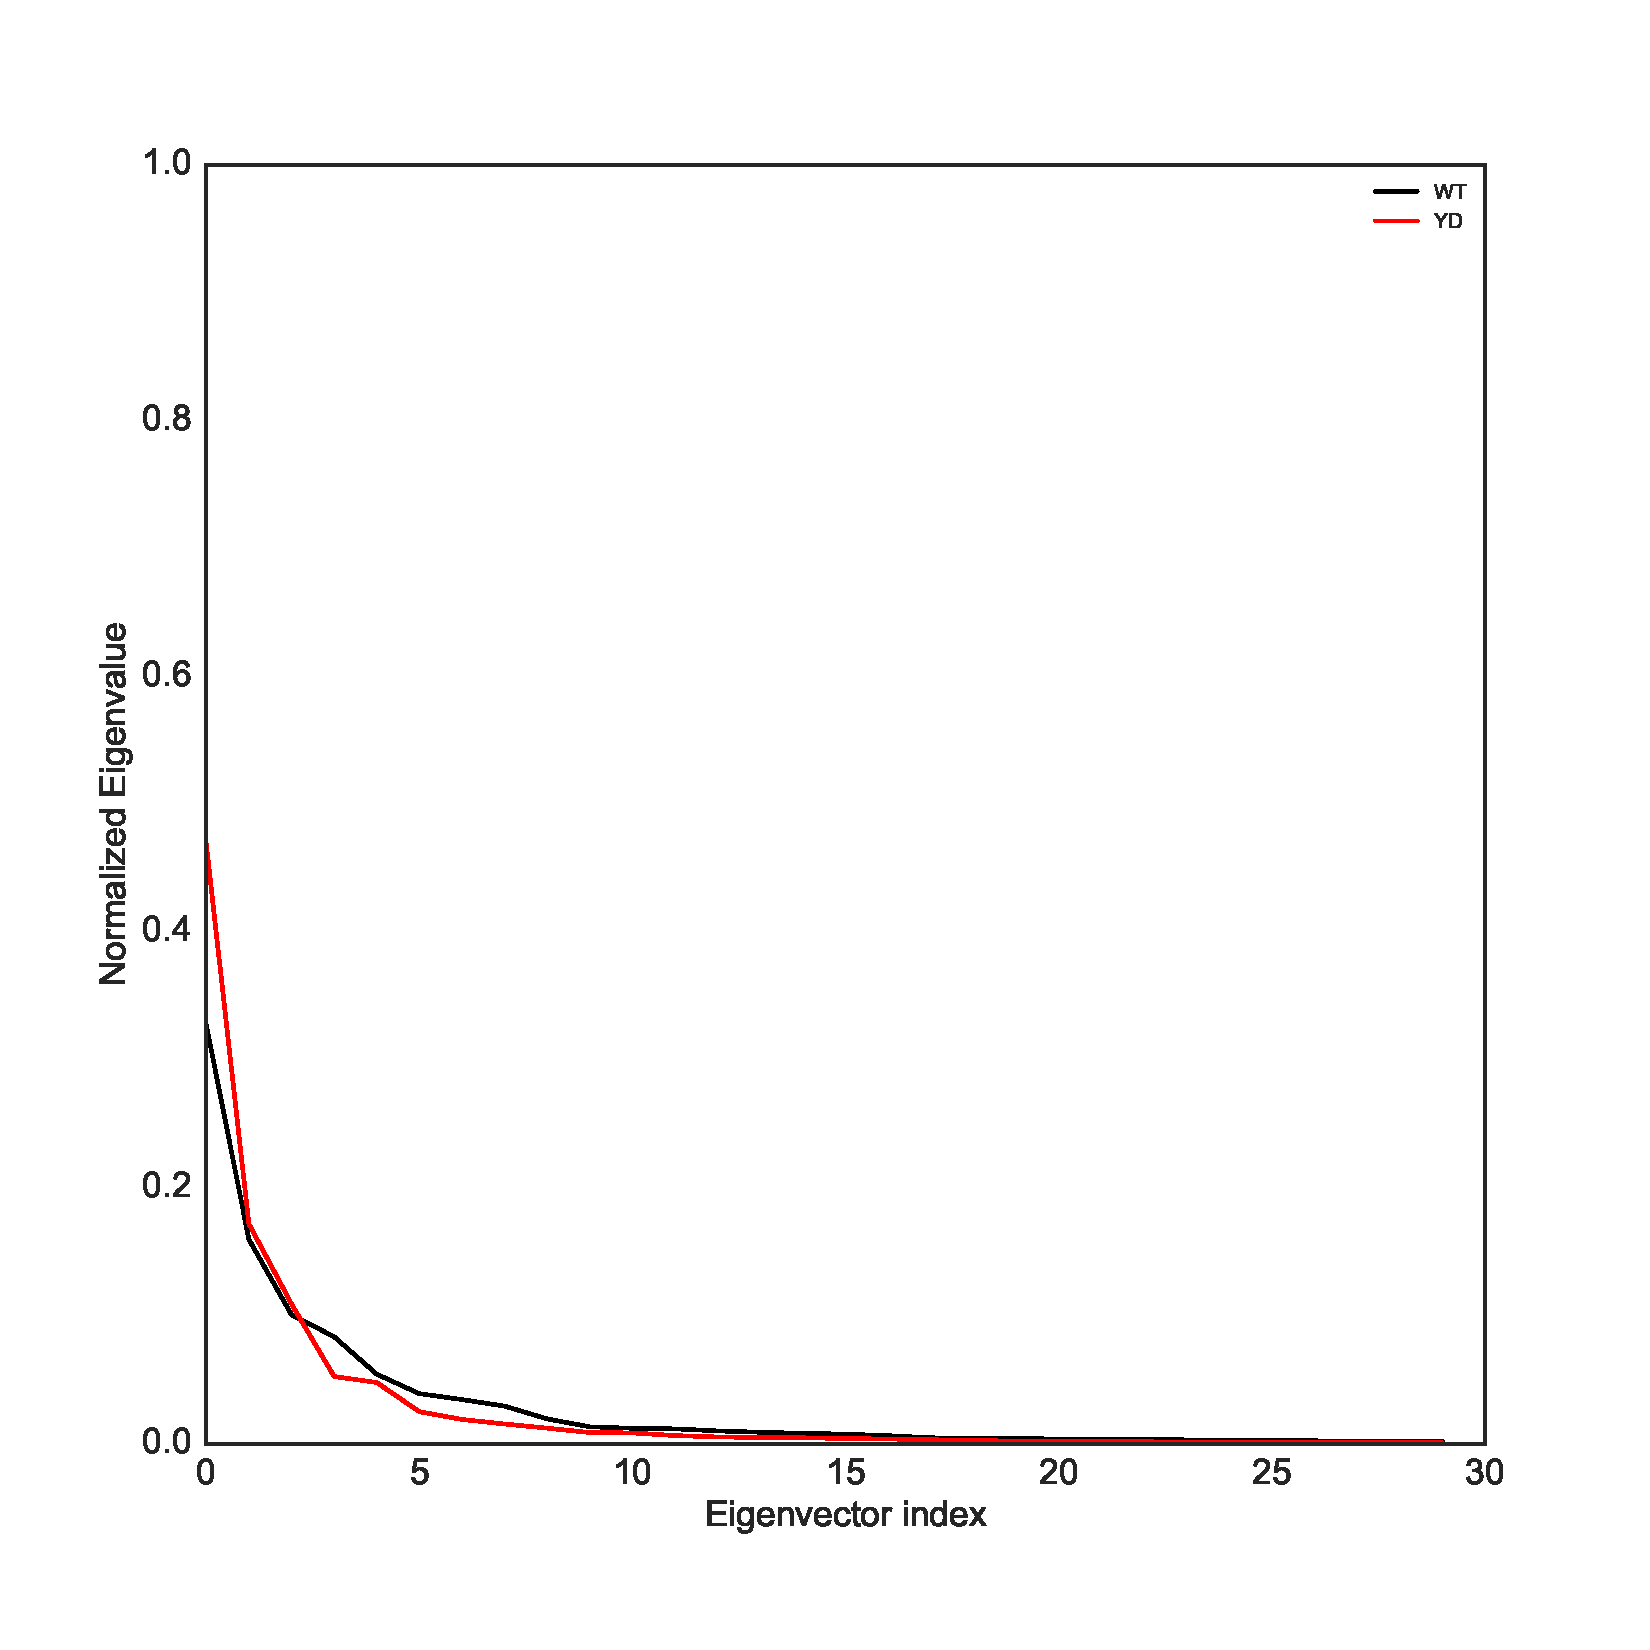
\includegraphics[height=0.35\textheight]{eigenvals}
	\FigureCaption{eigenvalues}
	\label{fig:eigenvalues}
\end{figure}
\todo{add 3 PC component projection}

\begin{figure}
	\thispagestyle{empty}
	\centering     %%% not \center
	\subfigure[WT]{\label{fig:a}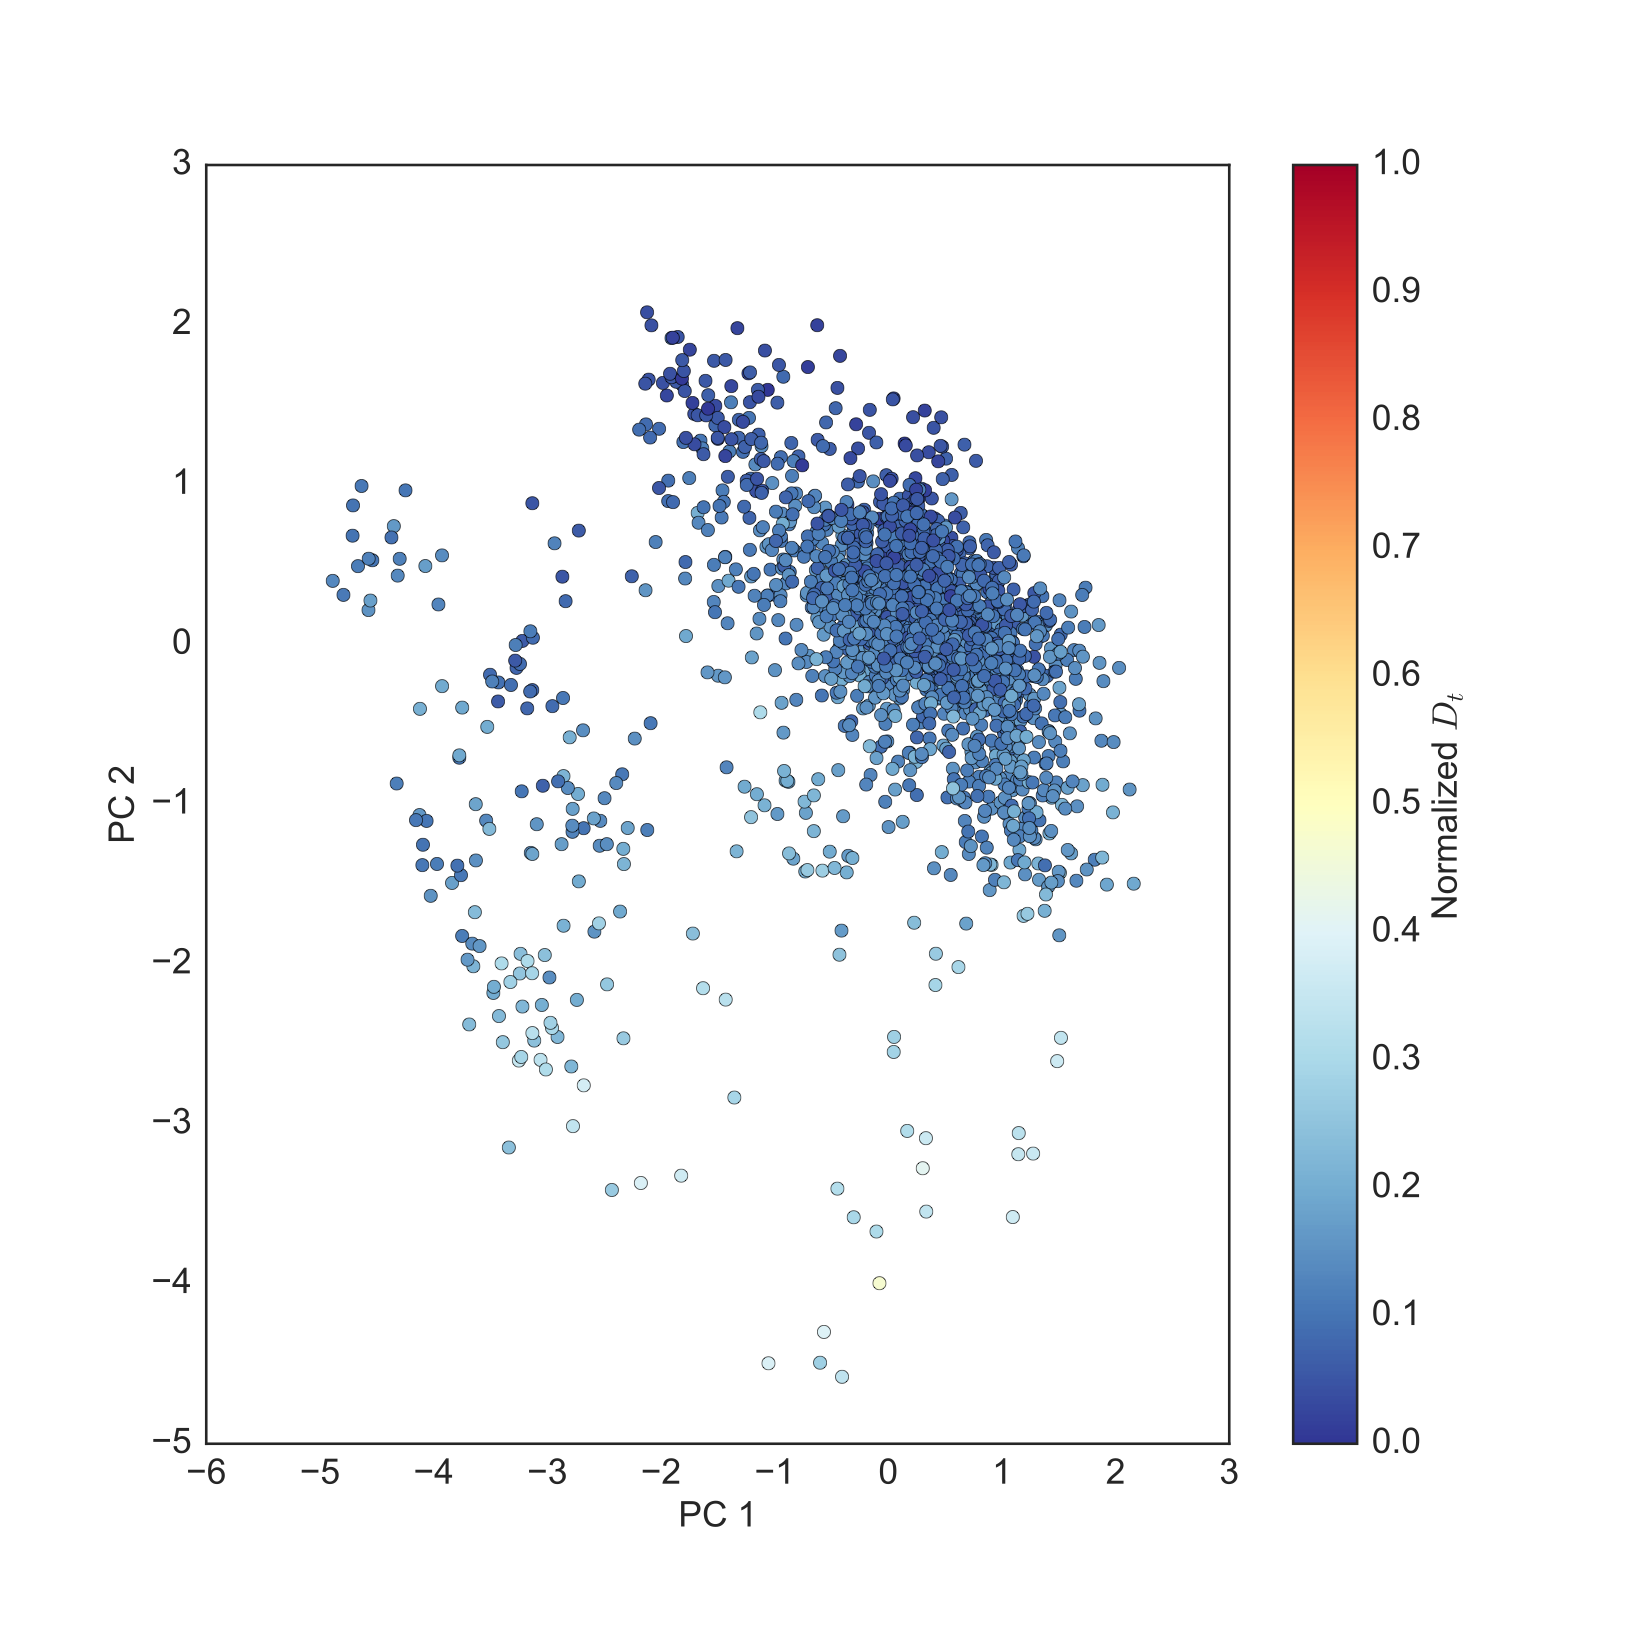
\includegraphics[width=0.49\textwidth]{2d_scatter_wt}}
	\subfigure[YD]{\label{fig:b}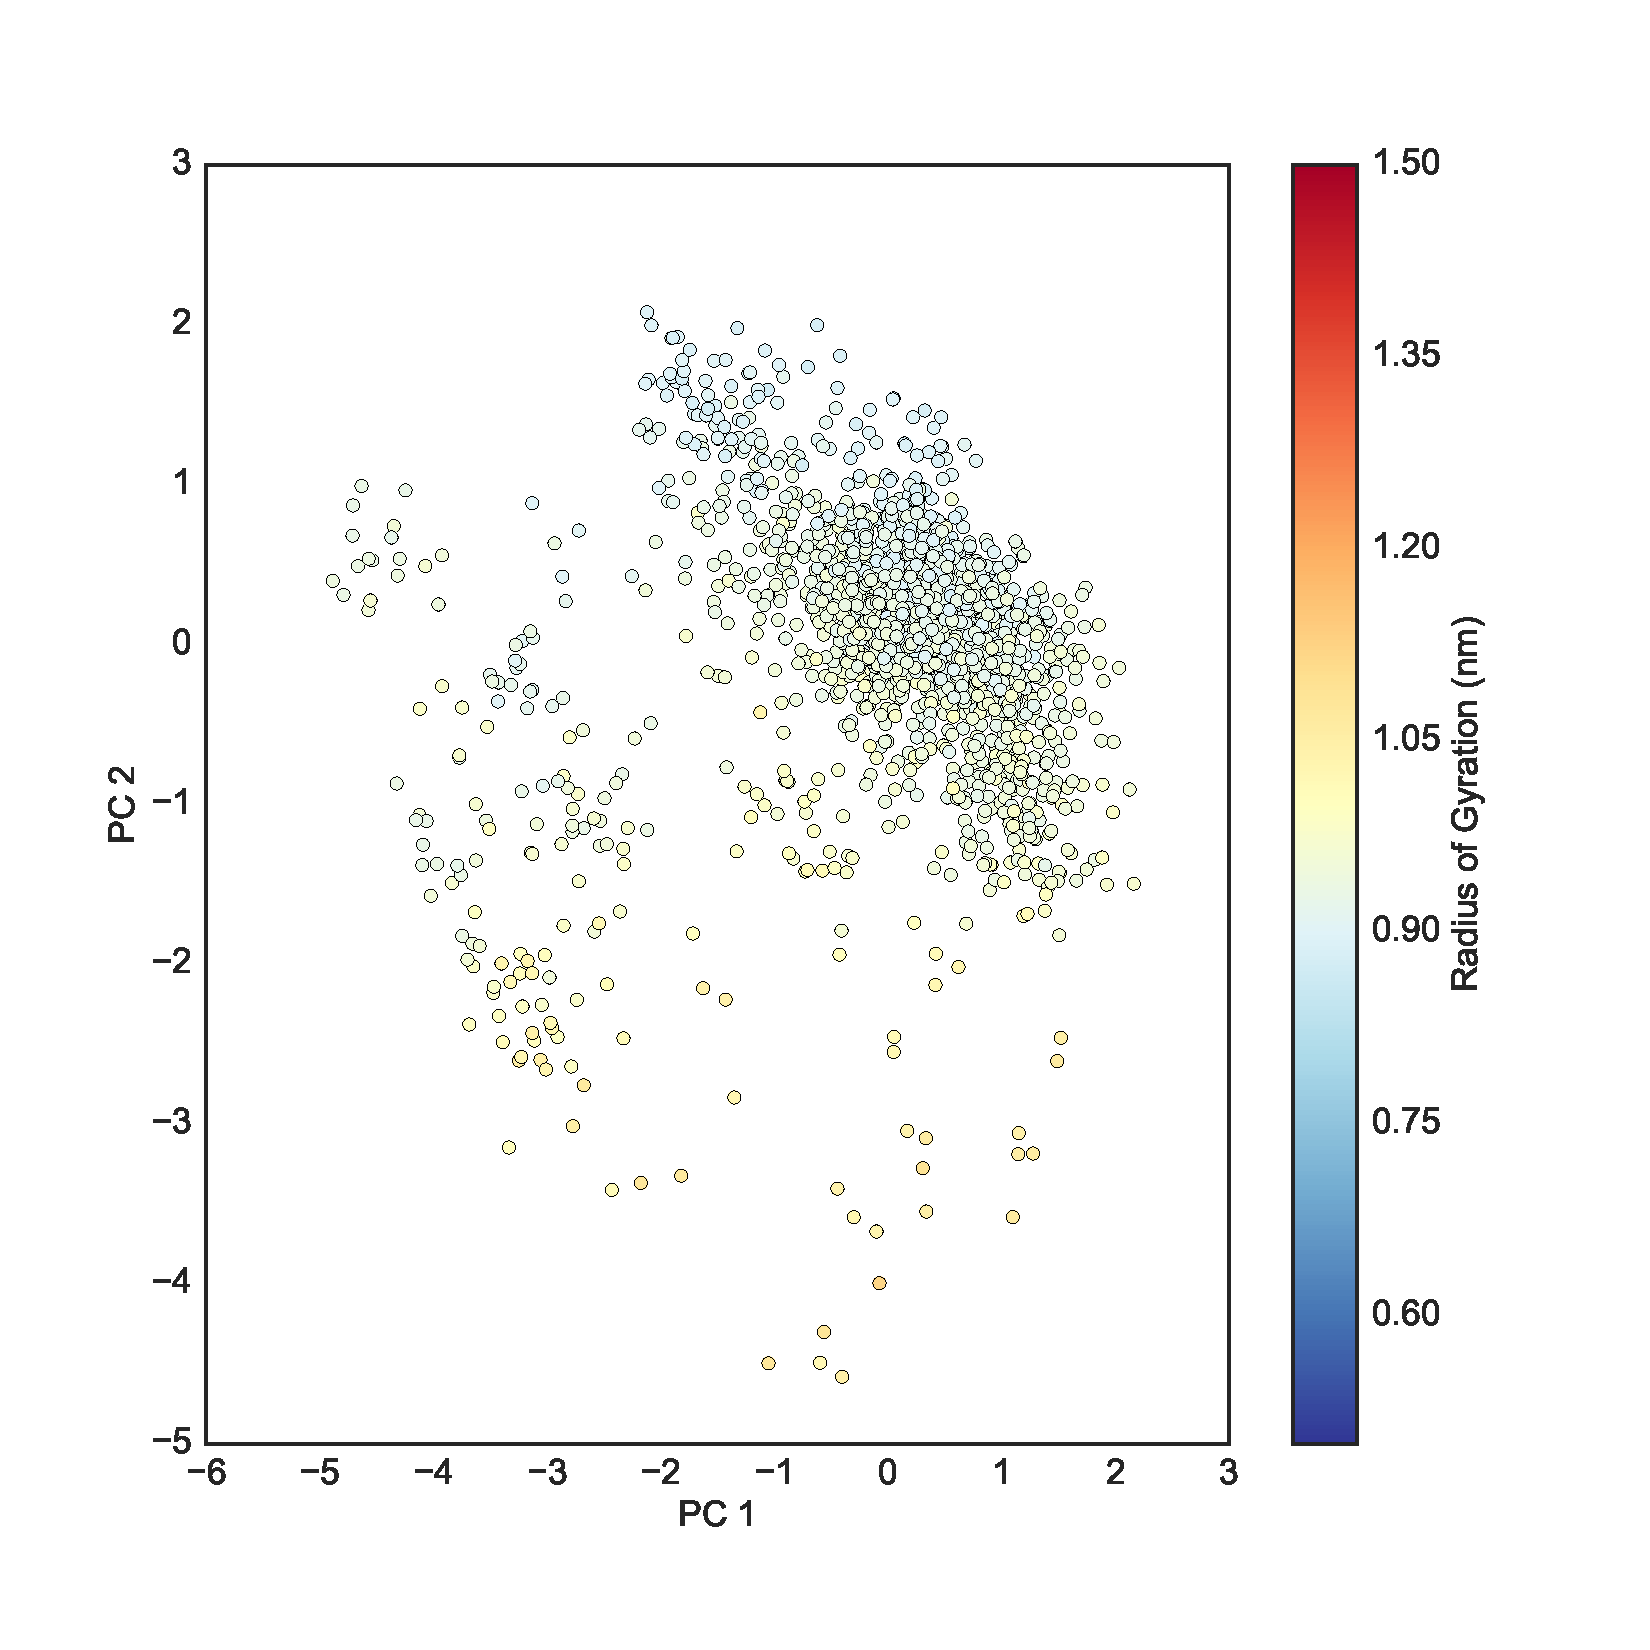
\includegraphics[width=0.49\textwidth]{2d_scatter_yd}} 
	\FigureCaption{Principal Component Analysis}{This is the text of the PCA figure}
	\clearpage
	\label{fig:pca}
\end{figure}




\begin{figure}
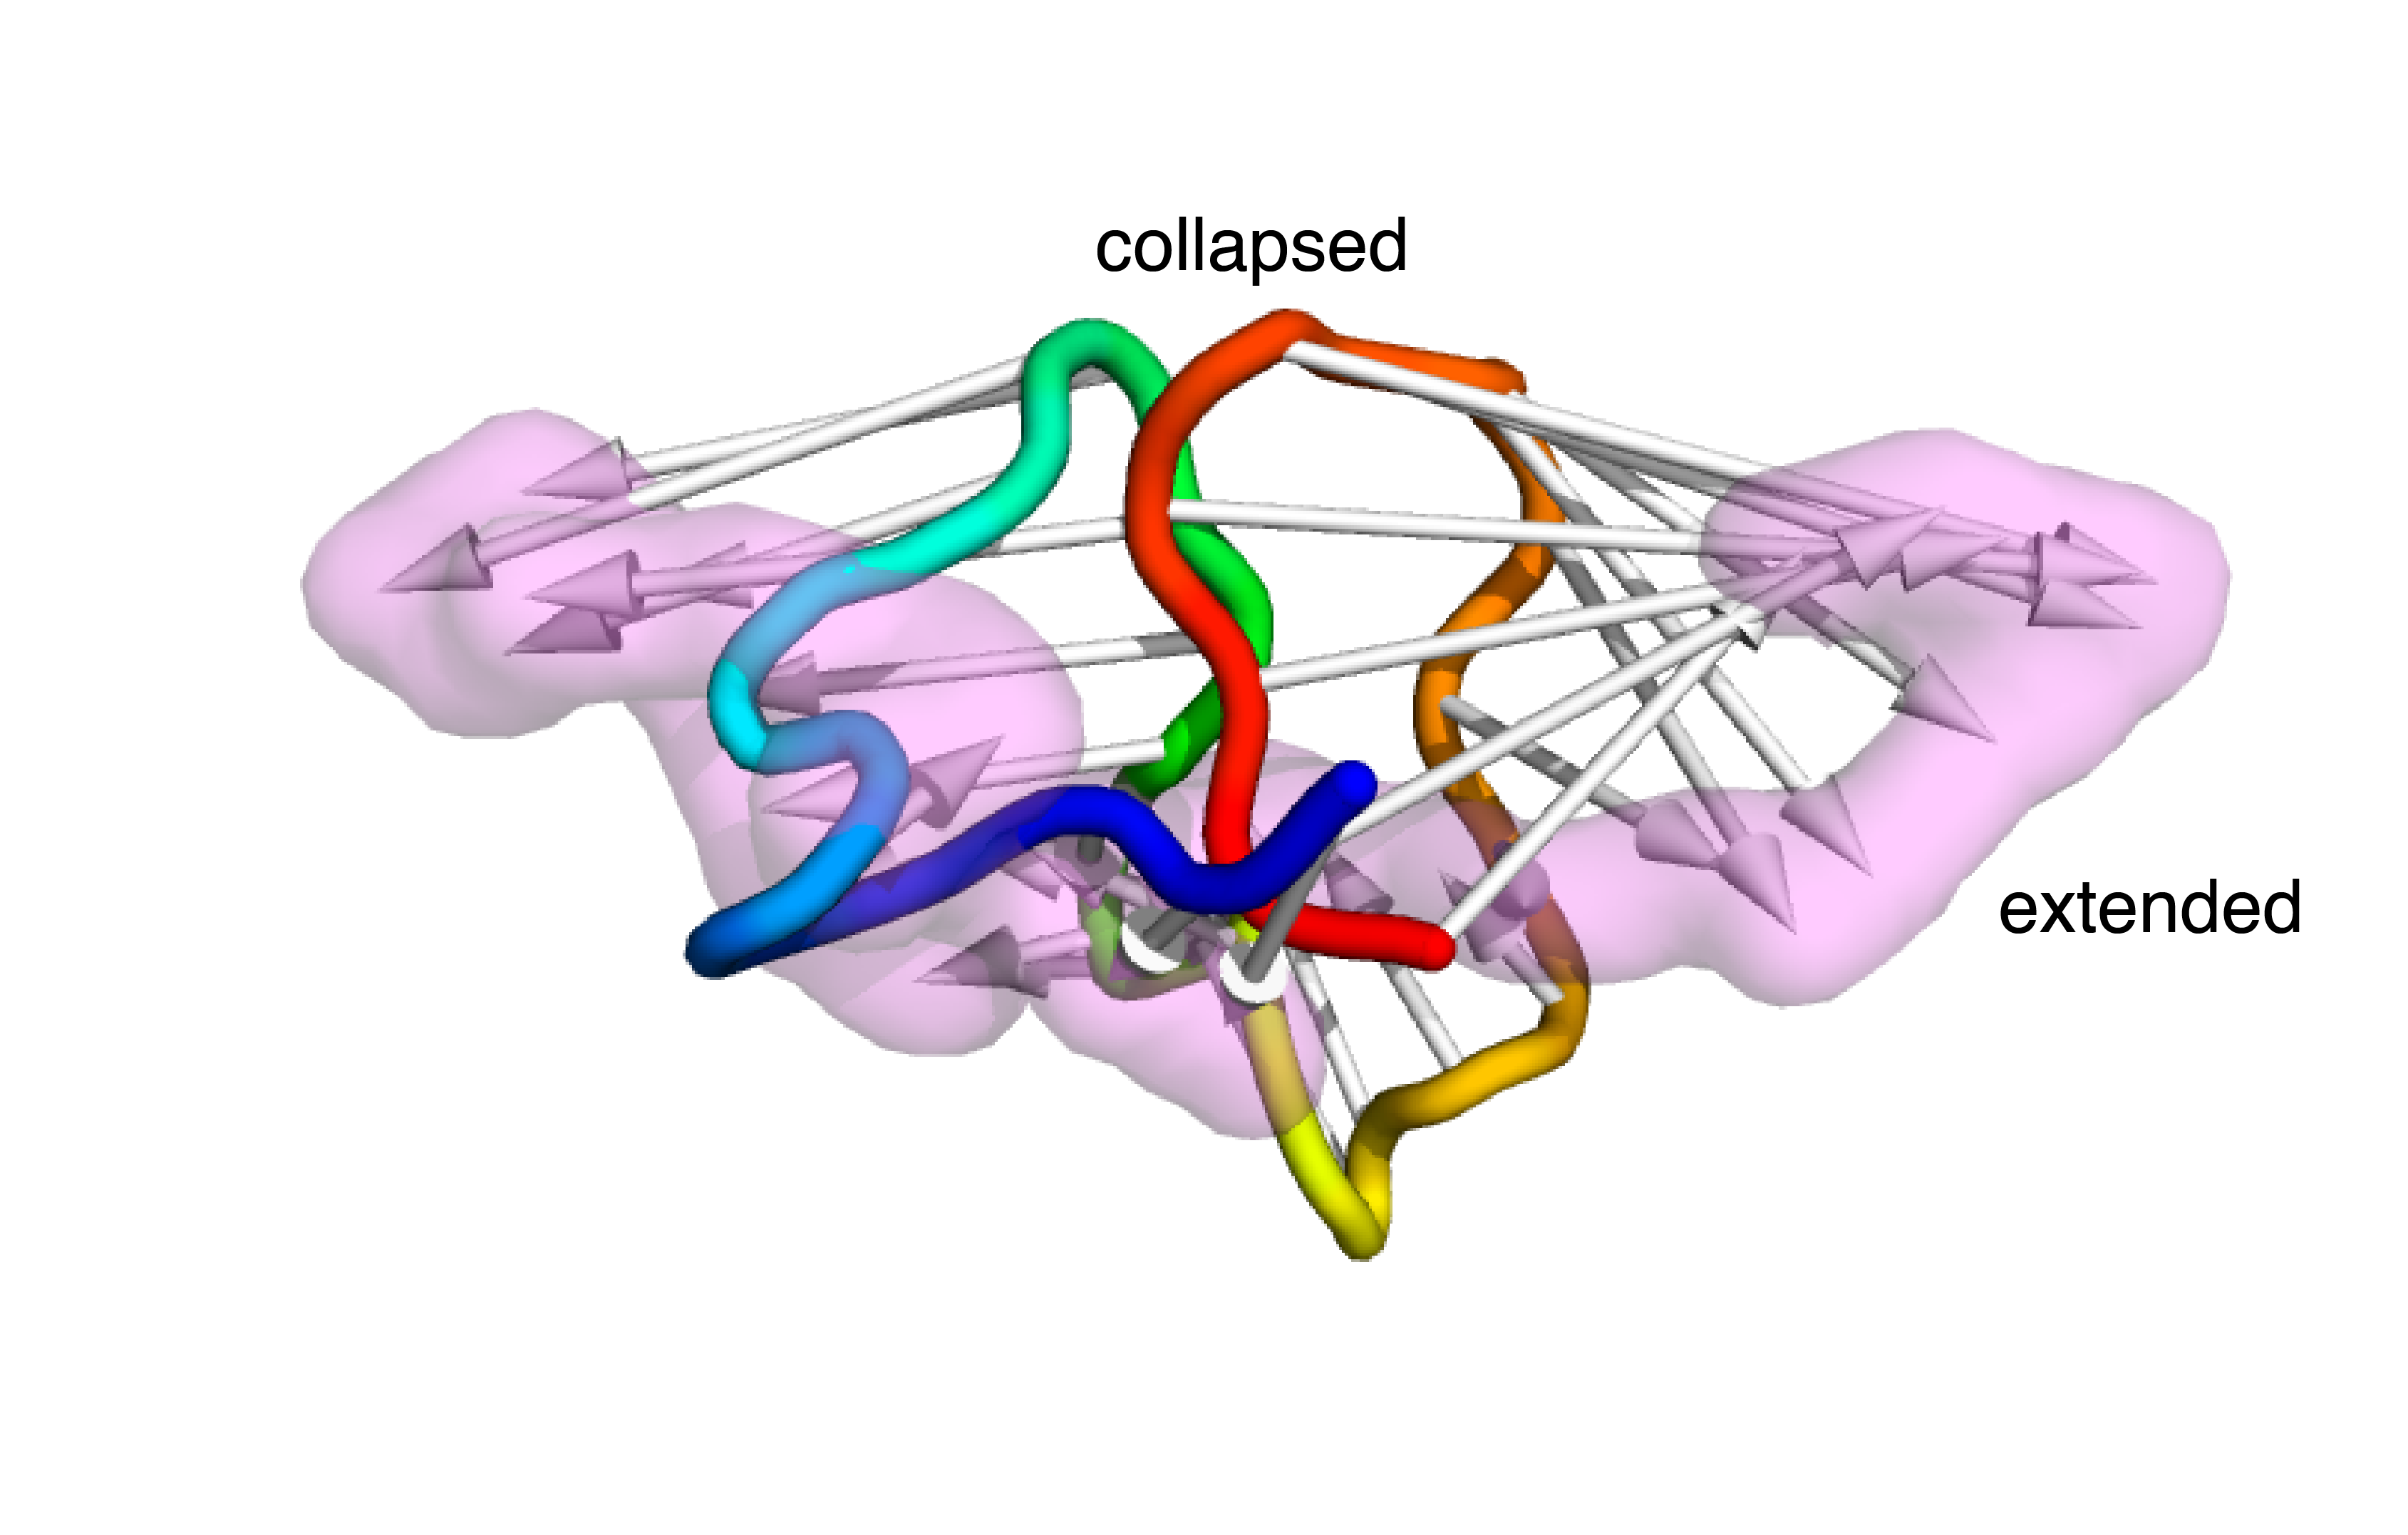
\includegraphics[height=0.4\textheight]{yd_porcupine}
\FigureCaption{porcupine plot}
\label{fig:porcupine}
\end{figure}  


\subsection{Whole protein simulations and conserved properties of \gct}

Our experimental analysis of the structural properties of the \gct using NMR and corresponding MDS are based on the properties of the WT and Y445D \gct polypeptides in isolation. In order to determine whether the conformations and dynamics we observed for the isolated ??CTs are physically consistent within the context of the full-length \tub protein, we docked the min-imum Ds \gct model (Fig. S9) onto the globular domain of an S.c. ?-tubulin homology model and used this as an initial structure for whole protein simulations on $\gamma$?tubulin. Due to the increase in system size, simulation times were reduced to 200ns.  As with the Y445D \gct polypeptide, the \gct in the whole protein simula-tion underwent exchange between extended and compact confor-mations (Fig. S10), suggesting both states are accessible in the presence of the globular domain. We found no contacts between residues in the globular domain with the 39 residues of the \gct throughout the 200 ns simulation (minimal distance between any pair of residues is > 0.7 nm). Structures for the full protein with the \gct at minimum radius of gyration (1.073 nm; model S11) and maximum radius of gyration (1.582 nm; model S12) are shown in Fig. 9A.


The CTs of $\alpha$- $\beta$- and \tub are enriched in acidic residues (Asp, Glu). \gct s across eukaryotes additionally contain clusters of hydrophobic or polar residues which are not found in $\alpha$- or $\beta$-CTs. Interestingly, the residues most broadened in Y445D NMR spectra, i.e. those most affected by the compact-to-extended transition (V15, D19, E20, A32, G34), are all found in positions conserved either on a sequence level or on a physical property level (polarity/charge) in a consensus \gct sequence(Fig. 9B). This suggests that clusters of hydrophobic residues, including those that contribute to transitions between compact and extended confor-mations in the S.c. D11 \gct, are a feature of an otherwise diverse set of \gct s across many eukaryotic organisms.


\section{Discussion}

Through NMR measurements and MD computer simulations, we demonstrate the first example of an IDP acting as a disorder-to-disorder regulatory switch and propose a physical mechanism to explain the regulation of an essential biological machine. 

Both NMR and MD are in strong agreement that the conformational sampling of the \gct lies entirely within the diordered ensemble as no signal of secondary structure was detected by either method. Diffusion measurements show that the major conformational state of the \gct in the WT and in the YD is collapsed, with the YD having a slightly larger hydrodynamic radius global average. However, NMR and MD simulations both provide evidence that a single point mutation to a negatively charged residue Y>D produces concerted motions along the entire polypeptide that are not present in the WT \gct. Analysis of the collective motions detected in MDS by PCA correspond closely to transitions between collapsed and extended states which leads us to hypothesize that the changes in chemical environment detected in MDS and difference in hydrodynamic radius is a product of an correlated opening and closing motion brought about by the Y>D mutation. This coordinated opening is likely brought about by the effects of electrostatic repulsion as the Asp substituion introduces further negative charge in an alread acidic region. It has been previously shown that charge has a strong influence on the conformational ensemble and diffusion rates in IDPs \cite{mao2010net}. Once the \gct enters the open state, several hydrophobic residues in the middle of the polypeptide(L464, A466, G468) become accessible for protein-protein interactions.

 Because both WT and YD appear to have the same collapsed native state and differ only when the YD undergoes transient excursion to an extended state, we can model this behaviour as a two well potential system \figref{fig:wellsb}. The equilibrium between extended and collapsed conformations is shifted by phosphorylation to render extensions more accessible in the YD.  Previously, such dynamics were only observed in the well characterized order-to disorder transitions, or the folding on binding paradigm. Furthermore, this model stands in contrast to the existing assumption that disordered ensembles are largely uniform \figref{fig:wellsa} and constitute a uniform space of random chains. And instead, we observe that the disordered ensemble has some structure that IDPs can explore to modulate functionality by giving rise to switch-like behaviour while remaining disordered. Such behaviour likely presents advantages to the cell through its ability to provide high specificity and low affinity binding at a low entropic cost. This suggests for the first time that the disordered conformational landscape can be organized and can therefore be host to coordinated and functional transitions.

\begin{figure}
\centering     %%% not \center
\subfigure[Figure A]{\label{fig:wellsa}\includegraphics[width=0.45\textwidth]{wells_a}}
\subfigure[Figure B]{\label{fig:wellsb}\includegraphics[width=0.49\textwidth]{wells_b}}
\label{fig:wells}
\end{figure}

From these findings we propose that phosphorylation at Y445 of the \gct acts as a regulatory switch to modulate protein-protein interactions. In order to better visualize this mechanism, we dock 3D structures obtained from full \tub simulations into cryo electron microscopy models of the $\gamma$-TuRC \figref{fig:turc} which previously lacked any information on the \gct due to its disordered nature. Based on this visualization we can propose a mechanism to explain the phenotype of hyper-stable microtubules in the Y445D mutants in vivo; the extensions that project outward from the complex brought about by the Y>D substitution, or phosphorylation, allow the $\gamma$-TuRC to selectively recruit effector proteins to the minus end of microtubules, making them available to the entire complex and which subsequently act to regulate microtubule dynamics. The constitutive addition of negative charge in the Y445D mutant therefore shifts the equilibrium between the collapsed and extended states, leading to a misregulation of the recruitment of microtubule associated proteins and thus a defect in microtubule dynamics. Which protein is being recruited by the \gct remains an open question but there are several candidates known to affect microtubule stability and localize to the spindle poles \todo{which candidates} are currently being verified through various experimental screens. However, the characterization of \gct conformational sampling  is an essential fist step in identifying potential interactors and understanding the complex mechanisms by which IDRs regulate large molecular machines.

\begin{figure}
\centering
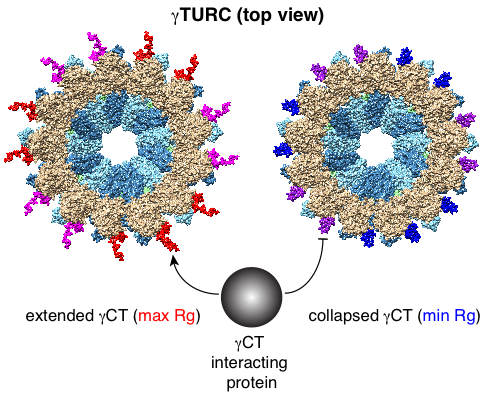
\includegraphics[height=0.5\textheight]{model}
\FigureCaption{$\gamma$-TuRC}
\label{fig:turc}
\end{figure}

\chapter{Conclusions}
\input{conclusion.tex}

%\input{appendix.tex}
\bibHeading{References}
\bibliography{thesis_cgo}
\bibliographystyle{plain}




\end{document}


 






